\documentclass[UTF8,12pt,a4paper,openany,fontset=none]{ctexrep}

\usepackage[a4paper,margin=2.35cm,headheight=15pt]{geometry}
\usepackage{graphicx}
\usepackage{booktabs}
\usepackage{longtable}
\usepackage{tabularx}
\usepackage{array}
\usepackage{enumitem}
\usepackage{xcolor}
\usepackage{amsmath,amssymb}
\usepackage{listings}
\usepackage{caption}
\usepackage{subcaption}
\usepackage{float}
\usepackage{fancyhdr}
\usepackage{hyperref}
\usepackage{tikz}
\usetikzlibrary{arrows.meta,positioning,shapes.geometric,fit}

\setCJKmainfont{Songti SC}
\setCJKsansfont{PingFang SC}
\setCJKmonofont{Songti SC}
\emergencystretch=2em
\Urlmuskip=0mu plus 1mu

\definecolor{TGBlue}{HTML}{245B78}
\definecolor{TGLightBlue}{HTML}{EAF3F8}
\definecolor{TGGold}{HTML}{B58B2A}
\definecolor{TGRed}{HTML}{A43D38}
\definecolor{TGGray}{HTML}{56616A}
\definecolor{TGCode}{HTML}{F5F7F8}

\hypersetup{
  colorlinks=true,
  linkcolor=TGBlue,
  urlcolor=TGBlue,
  citecolor=TGBlue,
  pdftitle={TwinGuide 双导管牙科导板半自动建模技术报告},
  % pdfauthor={TwinGuide 项目技术梳理}
}

\graphicspath{{figures/}}
\captionsetup{font=small,labelfont=bf,labelsep=quad}
\setlist{nosep,leftmargin=2em}
\setlength{\parindent}{2em}
\setlength{\parskip}{0.25em}
\renewcommand{\arraystretch}{1.25}

\pagestyle{fancy}
\fancyhf{}
\fancyhead[L]{TwinGuide 技术报告}
% \fancyhead[R]{研发技术汇报 / 项目交接}
\fancyfoot[C]{\thepage}

\lstset{
  basicstyle=\ttfamily\small,
  backgroundcolor=\color{TGCode},
  frame=single,
  rulecolor=\color{TGLightBlue},
  breaklines=true,
  columns=fullflexible,
  keepspaces=true,
  showstringspaces=false,
  keywordstyle=\color{TGBlue}\bfseries,
  commentstyle=\color{TGGray},
  stringstyle=\color{TGRed}
}

\newcommand{\projectpath}[1]{\nolinkurl{#1}}
\newcommand{\term}[1]{\textbf{#1}}
\newcommand{\risk}[1]{\textcolor{TGRed}{\textbf{#1}}}
\newcommand{\highlight}[1]{\textcolor{TGBlue}{\textbf{#1}}}

\newenvironment{takeaway}
  {\begin{center}\begin{minipage}{0.93\textwidth}\color{TGBlue}\hrule\vspace{0.5em}\textbf{注意：}\color{black}}
  {\vspace{0.5em}\color{TGBlue}\hrule\end{minipage}\end{center}}

\title{\Huge\bfseries TwinGuide 双导管牙科导板\\[0.35em]
自动建模技术报告\\[0.9em]
\Large 项目结构、建模流程、技术原理与风险梳理}
\author{面向研发技术汇报与项目交接}
\date{2026 年 7 月 27 日}

\begin{document}

\begin{titlepage}
  \centering
  \vspace*{2.6cm}
  {\color{TGBlue}\rule{\textwidth}{1.2pt}}\\[1.1cm]
  {\Huge\bfseries TwinGuide 双导管牙科导板\par}
  \vspace{0.4cm}
  {\Huge\bfseries 自动建模技术报告\par}
  \vspace{0.8cm}
  {\Large 项目结构、完整流程、建模方法与潜在难点\par}
  \vspace{1.0cm}
  {\color{TGBlue}\rule{\textwidth}{1.2pt}}\\[1.6cm]
  \begin{tabular}{rl}
    报告定位：& 研发技术汇报 / 项目交接\\
    案例主线：& 单颗缺失牙 tooth-47（FDI 47）\\
    资料范围：& TwinGuide 源码、配置、文档、测试及现有输出\\
    报告日期：& 2026 年 7 月 27 日
  \end{tabular}
  \vfill
  {\small 本报告只解释项目内部实际采用的方法，不扩展项目之外的临床或学术文献。\par}
\end{titlepage}

\pagenumbering{Roman}
\chapter*{报告说明与结论先行}
\addcontentsline{toc}{chapter}{报告说明与结论先行}

\section*{报告边界}

本报告面向研发人员、项目负责人和后续接手者，目标是回答三个实际问题：TwinGuide
当前能做什么、每一步为什么这样设计、继续开发时最容易在哪里出问题。报告以当前
工作区中的源码、病例配置、项目文档、测试和已有输出为唯一资料来源，不引入项目外
文献，也不把临床常识扩写为项目已经实现的功能。

所谓“完整阅读”，在本报告中指：盘点并阅读 \projectpath{src/twin_guide} 下全部
Python 模块，核对 \projectpath{docs}、\projectpath{tests}、\projectpath{examples}
与 \projectpath{data/cases}，并检查 tooth-47 的 JSON/YAML、过程报告、过程图和最终
STL。对 STL/PLY/GLB 等二进制网格采用拓扑、尺寸、体积和可视化检查，而非无意义的
逐字节解释。

\section*{结论先行}

TwinGuide 不是一个单纯“把几个 STL 做并集”的脚本。它已经形成了由
\term{病例语义、纯几何规划、Blender 实体化和独立结果检查}组成的分层流程：

\begin{enumerate}
  \item 从导套装配体的连通分量中识别真正具有轴孔的两根导管，并确定轴线、上下端和 C 口方向；
  \item 对牙列执行 FDI 牙位识别和导板映射，建立可用于“U 侧、背 U 侧、近远中和牙合方向”的局部语义坐标；
  \item 规划导孔、双导管操作窗和按牙位范围生成的轴扫掠观察窗；
  \item 在真实导管外壁与原始导板外壁上选择连接锚点，生成四根平滑主连接梁和可选 Y 型按压梁；
  \item 通过牙列净距裁剪、体素融合、精确差集、功能孔复切和手机运动包络差集，形成最终封闭 STL；
  \item 重新构建几何计划，对最终 STL 的拓扑、导管保留、梁连续性、孔道和观察窗进行检查。
\end{enumerate}

当前 tooth-47 是缺失下颌右侧第二磨牙 47 的黄金回归病例。现有结果 STL 为单一封闭
体，含 138,861 个顶点和 277,774 个三角面，体积约 $6670.72\,\mathrm{mm^3}$；观察窗
过程报告的全部 QA 项为真，手机包络也为封闭体。

\begin{takeaway}
项目的核心价值是把“牙位语义”和“几何建模”连成了可审计的数据流；当前最大工程风险
则是版本—产物追溯仍不充分、多个阶段仍标记为 experimental、布尔/体素过程成本高，
且手机避让尚未进入独立验证器的完整复算。
\end{takeaway}


\tableofcontents
\clearpage
\listoffigures
\clearpage
\listoftables
\clearpage

\pagenumbering{arabic}
\chapter{项目目标与目录结构}

\section{项目要解决的问题}

输入并不是一套已经可直接打印的双导结构，而是三个处于同一世界坐标系中的网格：
原始牙科导板、双导管装配体和患者牙列。程序需要保留导管装配关系，在导板上形成与
导管同轴的孔和足够的操作空间，再把导管、导板和新增梁架连接为一个可制造实体。

这项任务同时包含四类约束：

\begin{itemize}
  \item \term{功能约束}：导孔、C 口、操作窗和观察窗不能被融合重新堵住；
  \item \term{结构约束}：四根主梁、Y 梁及根部强化必须连续并与导板、导管可靠相交；
  \item \term{解剖约束}：梁和窗口的位置必须跟随牙弓语义，避免只依赖屏幕左右或固定 XYZ；
  \item \term{制造约束}：最终 STL 应闭合、流形、单一主要连通体，并控制孔道和净距。
\end{itemize}

\section{输入与 tooth-47 示例}

\begin{figure}[H]
  \centering
  \begin{subfigure}[t]{0.32\textwidth}
    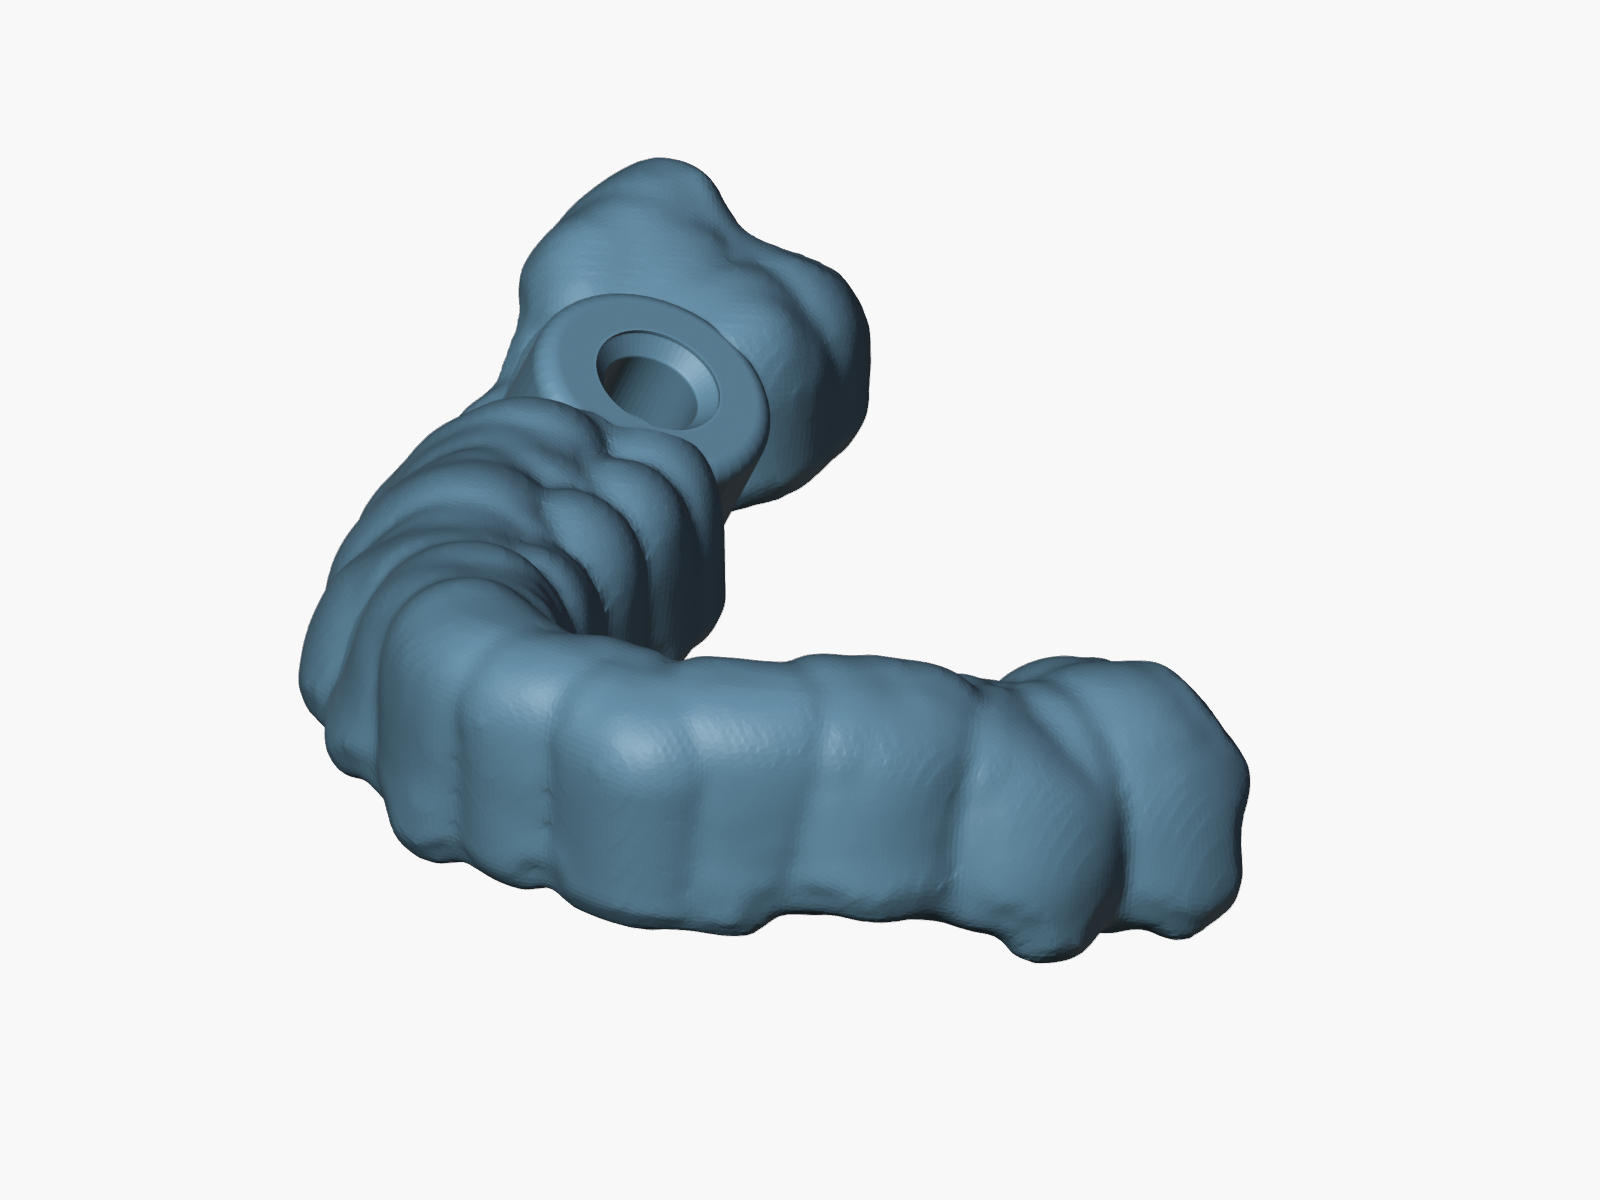
\includegraphics[width=\linewidth]{01_input_template.png}
    \caption{原始牙科导板}
  \end{subfigure}\hfill
  \begin{subfigure}[t]{0.32\textwidth}
    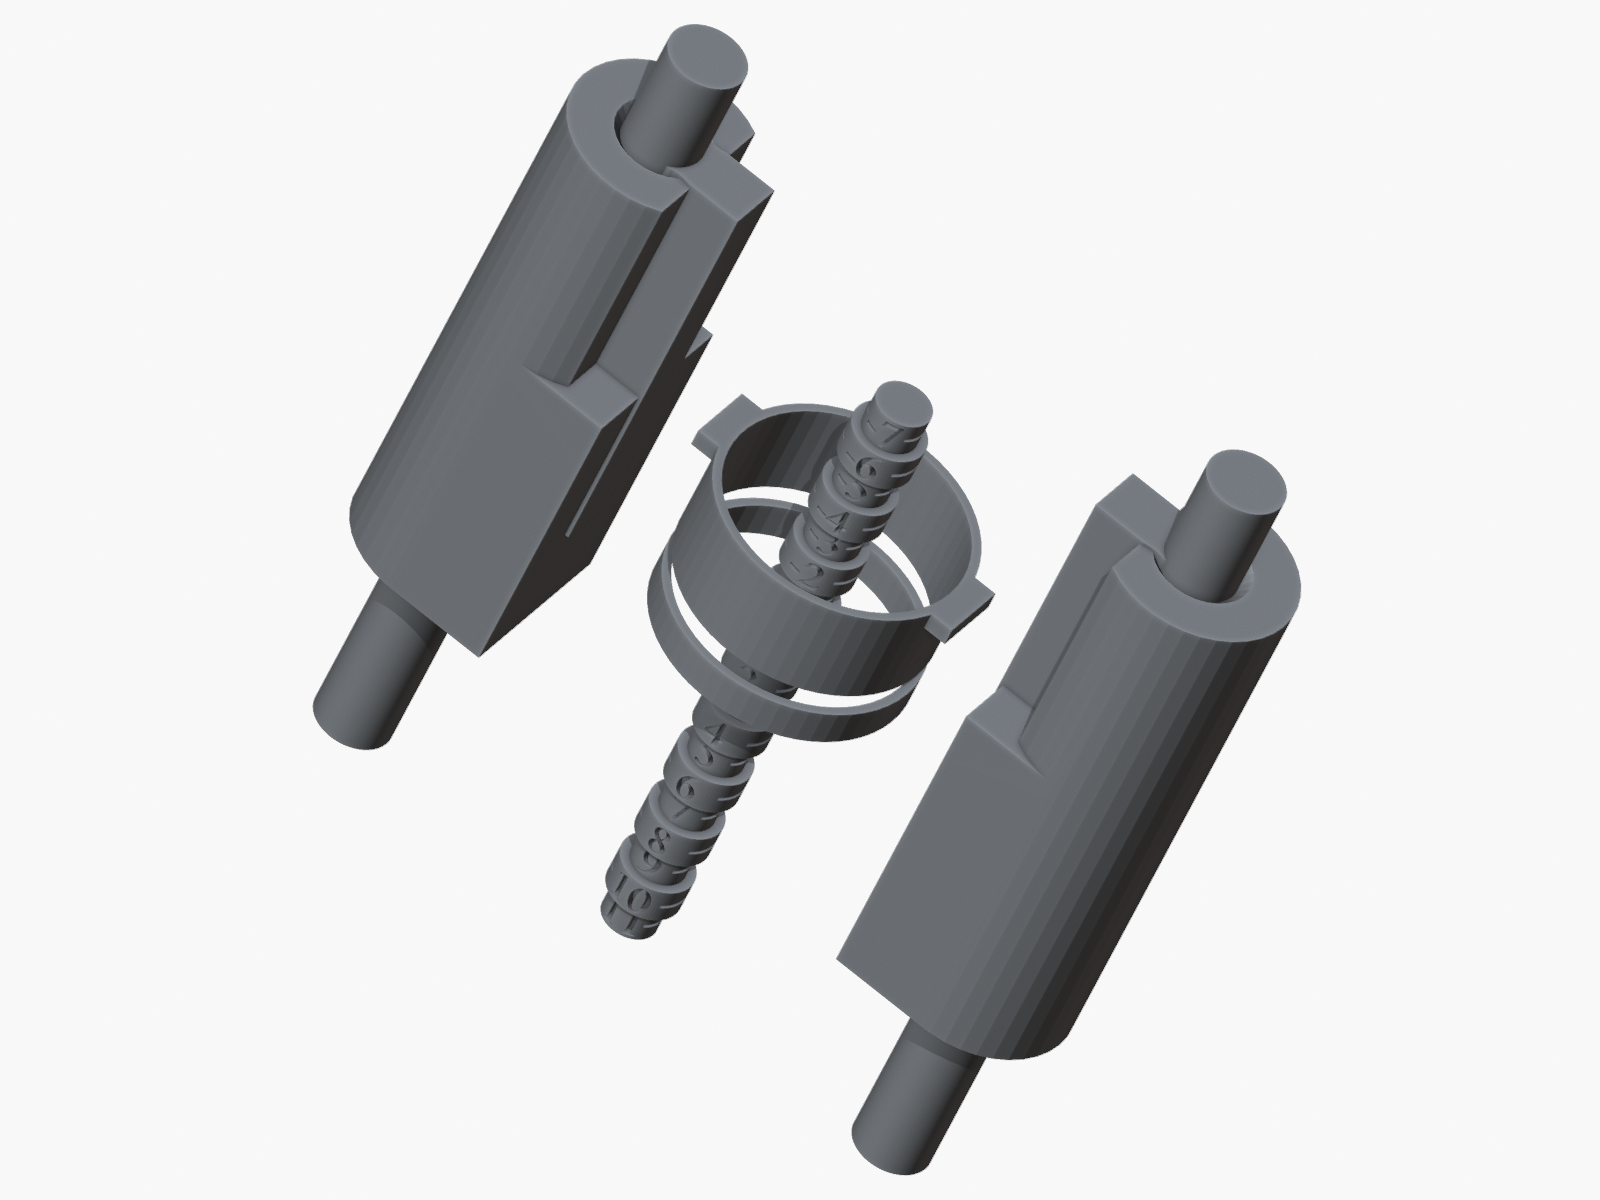
\includegraphics[width=\linewidth]{02_input_sleeves.png}
    \caption{双导管装配体}
  \end{subfigure}\hfill
  \begin{subfigure}[t]{0.32\textwidth}
    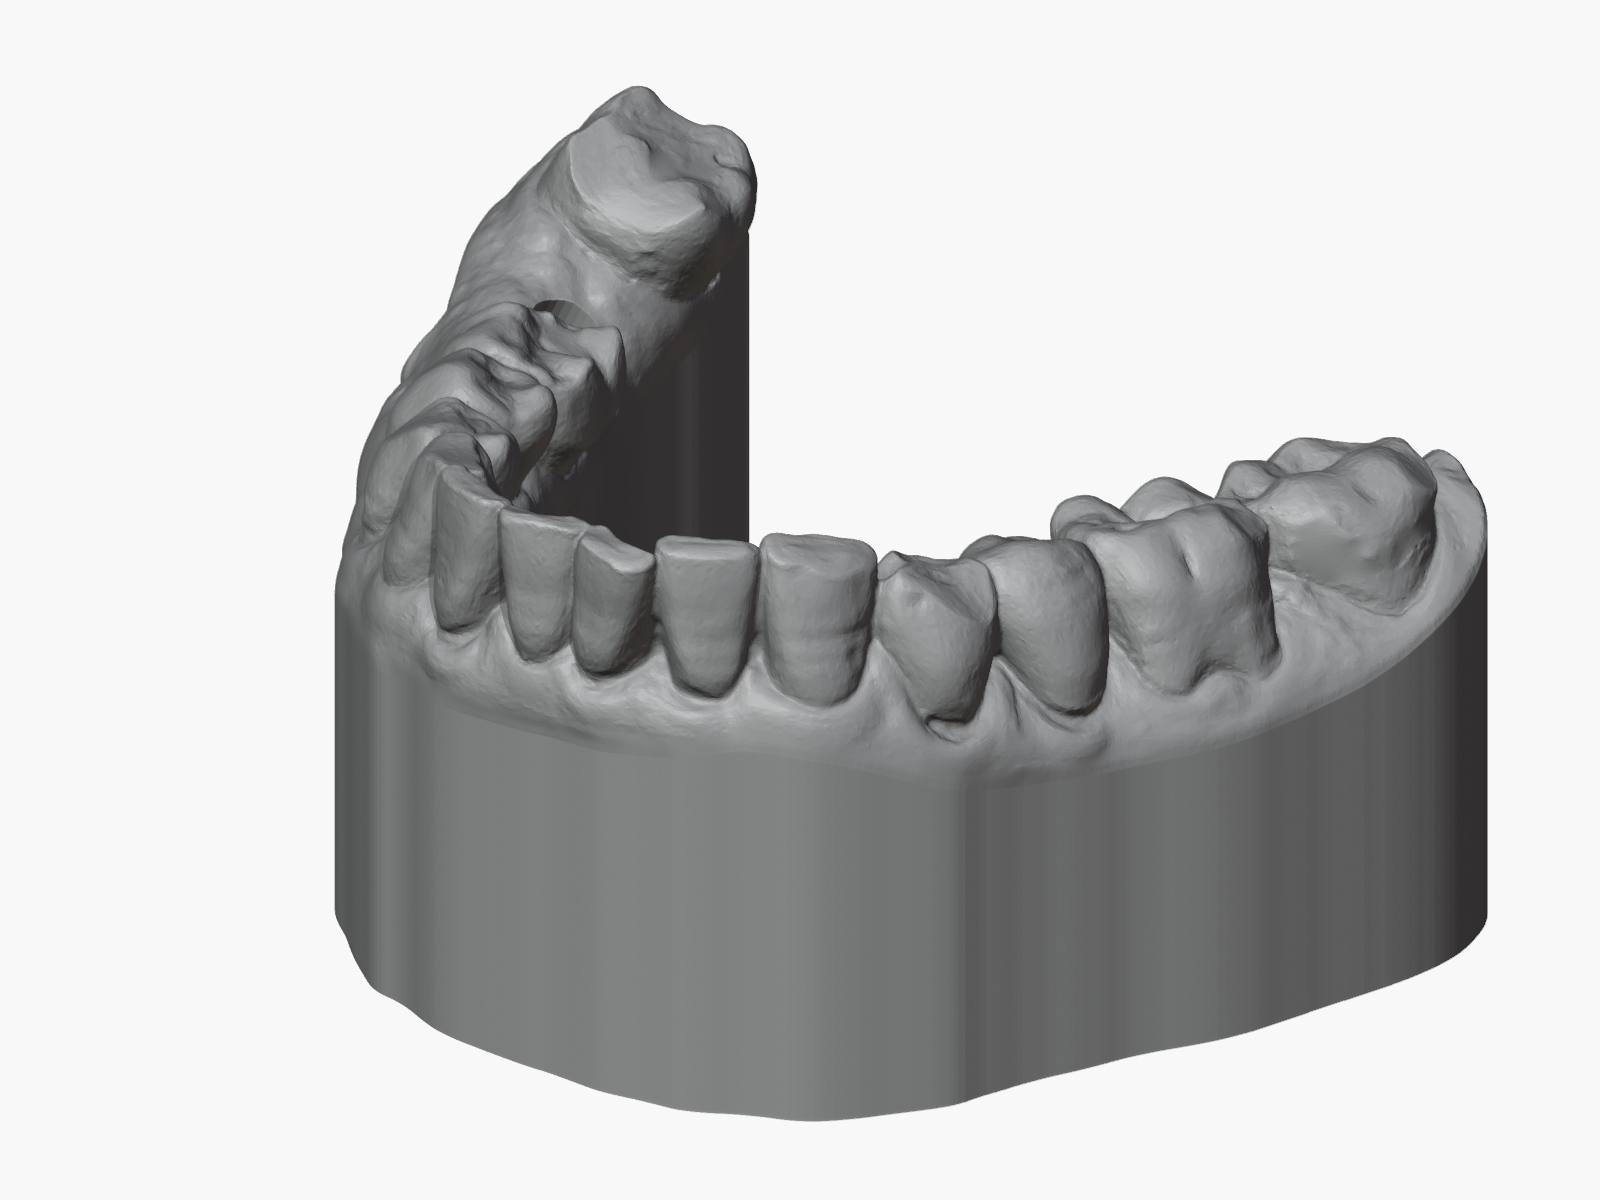
\includegraphics[width=\linewidth]{03_input_dentition.png}
    \caption{患者牙列/牙龈表面}
  \end{subfigure}
  \caption{tooth-47 的三类核心输入。三者必须采用相同坐标、毫米单位，并在导出 STL 前应用对象变换。}
  \label{fig:inputs}
\end{figure}

tooth-47 还配置了手机 STL、手机止挡报告及一个旧实验 cutter。当前正式流程把手机
STL 和止挡报告用于运动包络；旧 cutter 并不是主流程的权威观察窗来源。

\section{顶层目录及职责}

\begin{longtable}{p{0.28\textwidth}p{0.62\textwidth}}
  \toprule
  目录或文件 & 主要职责\\
  \midrule
  \endfirsthead
  \toprule
  目录或文件 & 主要职责\\
  \midrule
  \endhead
  \projectpath{src/twin_guide/} & 核心包：配置、阶段规划、几何算法、Blender 建模、验证与公开 API。\\
  \projectpath{src/twin_guide/blender/} & STL 读写、网格查询、布尔运算、圆管扫掠、体素融合、渲染和导出。\\
  \projectpath{src/twin_guide/sleeve_estimation/} & 导管轴线拟合、切片、圆拟合、参数化重建与网格完整性检查。\\
  \projectpath{data/cases/} & 规范病例输入和病例 YAML；按单颗与多颗病例分开。\\
  \projectpath{examples/} & 可执行 JSON 工程配置，负责输入路径、工程参数和输出位置。\\
  \projectpath{output/} & 过程 JSON、调试网格、渲染图和最终 STL。\\
  \projectpath{docs/} & 使用指南、七阶段流程、架构、配置和 API 文档。\\
  \projectpath{tests/} & 纯几何单元测试、Blender 后端测试、病例端到端测试和批量回归入口。\\
  \projectpath{run.py} & Blender 内的命令行启动脚本。\\
  \projectpath{blender-env.sh} & 将项目源码、工作区模块和局部依赖注入 Blender 5.2 Python。\\
  \bottomrule
\end{longtable}

\section{配置分层}

TwinGuide 刻意把配置分成两层。JSON 是可执行工程配置，保存 STL 路径、导管尺寸、梁径、
体素精度、手机避让和输出目录；病例 YAML 保存上下颌、牙位集合、观察窗范围、锚点站位、
Y 梁模式和人工审核状态。读取时，\texttt{CaseConfig.from\_json()} 以 JSON 所在目录解析
相对路径，再加载 YAML 并合并设计字段。

这种分层的优点是工程参数和病例语义互不混淆；代价是必须维护二者的一致性。代码通过
拒绝未知字段、拒绝 YAML 重复键、拒绝 JSON/YAML 对同一设计字段重复定义等方式降低歧义。

\section{运行入口}

\begin{lstlisting}[language=bash,caption={当前项目的三个主要命令}]
./blender-env.sh --background --python run.py -- \
  process --config examples/case-tooth-47.json

./blender-env.sh --background --python run.py -- \
  generate --config examples/case-tooth-47.json --validate

./blender-env.sh --background --python run.py -- validate \
  --config examples/case-tooth-47.json \
  --model output/tooth_47/twin_guide.stl
\end{lstlisting}

\texttt{process} 只执行几何规划；\texttt{generate} 再把规划实体化并导出；
\texttt{validate} 读取最终 STL，重新建立预期几何并进行独立检查。生产生成还会检查 YAML
中的 review 状态，显式为 pending、unreviewed 等状态时默认停止。


\chapter{软件架构与数据流}

\section{分层结构}

项目的结构可以概括为“配置与语义层—规划层—实体化层—验证层”。

\begin{figure}[H]
\centering
\begin{tikzpicture}[
  node distance=8mm and 11mm,
  box/.style={draw=TGBlue,rounded corners,fill=TGLightBlue,minimum height=10mm,
    text width=3.35cm,align=center,font=\small},
  arrow/.style={-{Latex[length=2.2mm]},thick,color=TGBlue}
]
  \node[box] (cfg) {JSON 工程配置\\YAML 病例语义};
  \node[box,right=of cfg] (analysis) {病例分析\\导管与牙位语义};
  \node[box,right=of analysis] (plan) {七阶段几何规划\\GenerationContext};
  \node[box,below=of plan] (mesh) {Blender / Trimesh\\实体化与布尔运算};
  \node[box,left=of mesh] (stl) {最终 STL\\过程图与 JSON};
  \node[box,left=of stl] (qa) {独立重建期望\\ValidationResult};
  \draw[arrow] (cfg) -- (analysis);
  \draw[arrow] (analysis) -- (plan);
  \draw[arrow] (plan) -- (mesh);
  \draw[arrow] (mesh) -- (stl);
  \draw[arrow] (stl) -- (qa);
  \draw[arrow,dashed] (cfg) |- (qa);
\end{tikzpicture}
\caption{TwinGuide 的主要数据流。规划结果先以数据类保存，实体化阶段才创建网格。}
\label{fig:architecture}
\end{figure}

\subsection{配置与公共类型}

\projectpath{config.py} 定义 \texttt{CaseConfig} 及全部参数数据类；
\projectpath{models.py} 保存导管、导板标架、切割体和输出类型；
\projectpath{types.py} 定义阶段状态和 \texttt{GenerationContext}。这些类型承担了模块间
契约，使上游结果不会通过隐式全局变量传给下游。

\subsection{纯几何规划}

规划层以点、向量、曲线和文件路径作为主要输出。它负责决定“在哪里切、在哪里连、中心线
怎么走”，尽量不在此阶段执行复杂布尔。这样锚点错误可以在调试图中直接看到，而不会被
体素化或网格修复掩盖。

\subsection{实体化与布尔层}

\projectpath{blender/mesh_builders.py} 把圆柱、窗口和中心线转换为封闭网格；
\projectpath{blender/guide_modeling.py} 组织牙列裁剪、体素融合和复切；
\projectpath{blender/booleans.py} 封装 Blender 多求解器和 manifold3d 精确差集。

\subsection{验证层}

\projectpath{guide_validation.py} 不直接相信生成时的对象，而是读取导出的 STL，重新运行
病例分析、牙位映射、切口规划和连接规划，然后以 BVH 查询、中心线采样和拓扑统计检查结果。
这种“重新建立期望”的方式比仅检查文件存在更有价值，但仍有后文所述的覆盖空白。

\section{七个正式阶段与实际实体化步骤}

\begin{table}[H]
\centering
\small
\begin{tabularx}{\textwidth}{c p{0.22\textwidth} X p{0.16\textwidth}}
  \toprule
  阶段 & 名称 & 主要输出 & 代码成熟度\\
  \midrule
  1 & 导管识别与位姿分析 & 两根当前模式导管、导板局部标架 & stable 1.0\\
  2 & 牙位识别 & FDI 映射、牙弓方向、观察窗语义轴 & experimental 0.4\\
  3 & 窗口规划 & 导孔、操作窗、观察窗 cutter & experimental 0.2\\
  4 & 联建锚点 & 导管 Q/P、导板 A 点及配对 & experimental 0.1\\
  5 & 按压梁选点 & 三锚点、Y 汇合点与强化参数 & experimental 0.1\\
  6 & 结构连接 & 四根主梁、Y 梁和特殊梁中心线 & experimental 0.1\\
  7 & 净距调整 & 手机左右摆动封闭包络 & experimental 0.1\\
  \bottomrule
\end{tabularx}
\caption{\texttt{generation\_process.py} 中声明的七阶段。}
\end{table}

七阶段结束后，\texttt{generate\_guide()} 才调用实体化入口。因此“第 7 阶段完成”不等于
STL 已经生成；它只表示所需包络或几何计划已经准备好。真正的切割、融合、导出和渲染发生
在 \texttt{build\_guide\_from\_links()}。

\section{坐标与单位约定}

全部几何使用世界坐标和毫米。局部标架只用来排序、区分方向和构造参数化几何：

\begin{itemize}
  \item \texttt{TemplateFrame.normal} 指向导板牙合外侧；
  \item \texttt{lateral} 与 \texttt{depth} 描述导板局部横向和深度；
  \item 牙位映射给出 \texttt{e\_occ}、每牙 \texttt{local\_tangent} 和
    \texttt{local\_outward}；
  \item 导管轴在病例分析后统一为从 C 口高端指向闭合孔低端。
\end{itemize}

如果输入网格坐标不一致，或轴符号没有被正确统一，后续每个“上/下、内/外、近/远”的
判断都会同时出错。因此项目在牙位和导管阶段均采用失败关闭，而不是继续猜测。


\chapter{端到端建模流程与技术原理}

本章按程序真正的数据依赖顺序说明算法。为便于交接，每一节均回答“目的、核心方法、设计
理由、输出和主要失败条件”，公式只保留理解实现所必需的部分。

\section{步骤一：病例加载、表面采样与导管识别}

\subsection{病例加载与公共几何}

\texttt{analyze\_case()} 清空 Blender 场景后导入导板、牙列和一个或多个导管装配体。
导板和牙列表面被采样为带法向和面索引的 \texttt{SurfaceSample}。导板中心优先使用封闭
网格的体积重心；如果计算出的重心落在包围盒外，则退化为表面样本均值。

导板局部法向由表面点云主平面确定。若点云中心为 $\bar{\mathbf p}$，协方差矩阵为
\[
  \mathbf C=\frac{1}{N}\sum_i
  (\mathbf p_i-\bar{\mathbf p})(\mathbf p_i-\bar{\mathbf p})^\mathsf T,
\]
最小特征值对应的特征向量近似为导板法向。程序再用上下颌或 YAML 中确认的牙合轴统一
法向符号。

\subsection{为什么先检查真实轴孔}

导管装配体可能包含导管、连接附件和实心 cutter。如果只按“长度和直径最像导管”打分，
实心圆柱也可能获胜。当前实现先对每个连通分量拟合轴线，并在轴向 15\%、25\%、35\%、
50\%、65\%、75\%、85\% 七处取探针点。点位于实体外部表示该处处在孔腔中，七点的通过
比例必须至少为 0.60。

只有通过孔道门槛的候选才会两两组合。候选对评分主要考虑：
\[
  E_{\mathrm{size}}=
  \sum_{j=1}^{2}\left(
  \frac{|H_j-H_0|}{H_0}+\frac{|R_j-R_0|}{R_0}\right),
  \qquad
  E_{\mathrm{axis}}=1-|\mathbf a_1\cdot\mathbf a_2|.
\]
代码按尺寸误差、轴线不平行误差、导管间距和组件索引依次排序，选择最优对。尺寸只在
已经确认有孔的候选中排序，不能让实心 cutter 反超。

\subsection{轴线与 C 口方向}

导管轴线不是只对全部顶点做一次 PCA。\projectpath{sleeve_estimation} 会对网格切片，
从内孔截面拟合圆和直线，以孔道证据修正主轴。轴向上下端再由顶点投影范围和端部拓扑
确定。两根导管中心连线投影到各自轴线法平面：
\[
  \mathbf c_i=
  \operatorname{normalize}\!\left[
  (\mathbf o_j-\mathbf o_i)-
  \mathbf a_i\big((\mathbf o_j-\mathbf o_i)\cdot\mathbf a_i\big)
  \right],
\]
所得 $\mathbf c_i$ 指向另一根导管，作为 C 口方向；其反方向用于放置主梁接触点。

\subsection{input 与 generated 两种导管模式}

\begin{table}[H]
\centering
\small
\begin{tabularx}{\textwidth}{p{0.18\textwidth}XX}
  \toprule
  对比项 & generated & input\\
  \midrule
  最终导管来源 & 按识别位姿和八个解析尺寸重建 & 保留识别出的输入导管分量\\
  锚点表面 & 参数化外壁 & 真实输入外壁射线命中\\
  导孔处理 & 全体融合后权威复切 & 导管加入前只复切基础体\\
  低梁嵌入 & 可全直径预埋，依赖后续复切 & 最多约 1.45 mm，并受真实壁厚限制\\
  连通体清理 & 复切后保留最大连通体 & 只删除小于 0.25 个体素的数值碎片\\
  主要优势 & 尺寸一致、对扫描噪声不敏感 & 保留真实导管形态和既有孔腔\\
  主要风险 & 重建参数与实际零件可能不一致 & 输入缺陷被保留，体素融合仍会离散化表面\\
  \bottomrule
\end{tabularx}
\caption{两种导管实体模式的布尔顺序差异。}
\end{table}

两种模式共享同一套识别位姿、C 口语义和下游规划。这个设计避免为不同导管来源复制整套
流程，但也要求每个涉及孔道的步骤明确知道当前模式。

\section{步骤二：牙位识别、FDI 编号与导板映射}

\subsection{从三维牙列到二维牙弓证据}

TwinGuide 通过工作区中的 \projectpath{tooth_guide_mapping} 模块执行牙位工作流。流程先把
牙冠表面投影到患者左右—前后平面，组合四类证据：连续三角形轮廓、最高表面高度、插值
法向和融合解剖边缘。图 \ref{fig:projection} 展示了 tooth-47 的实际输出。

\begin{figure}[H]
  \centering
  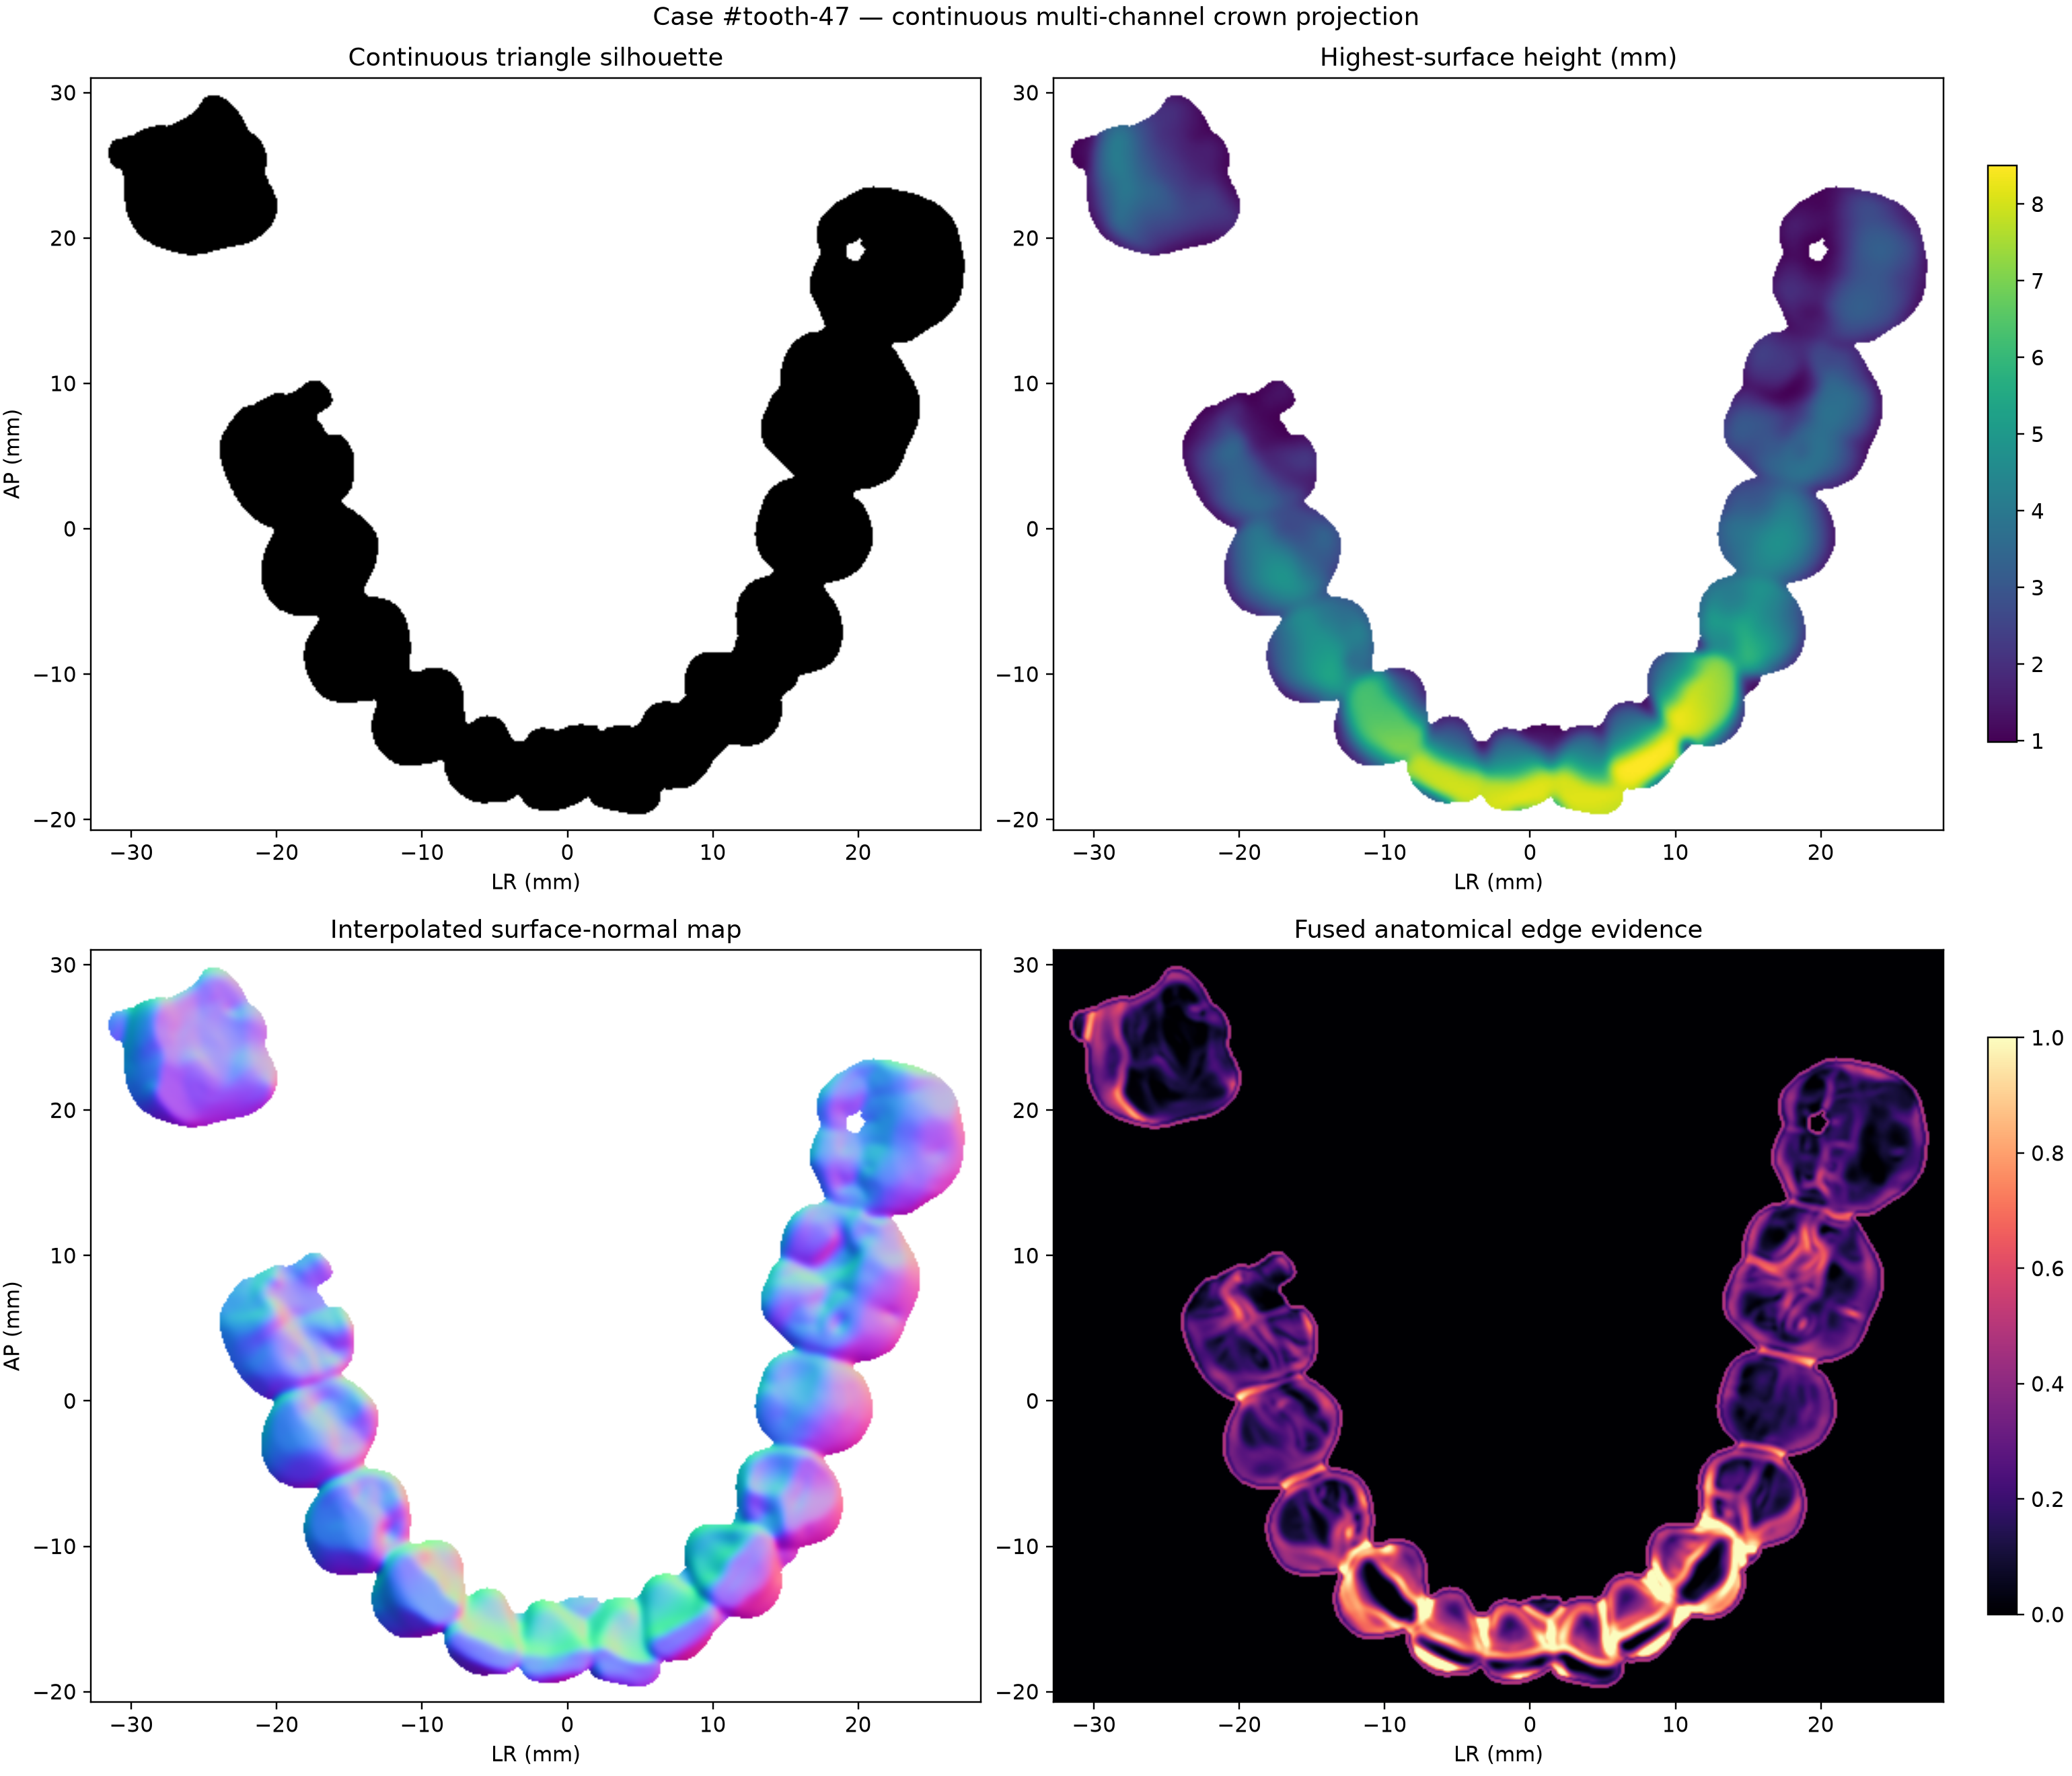
\includegraphics[width=0.96\textwidth]{04_multichannel_projection.png}
  \caption{tooth-47 多通道牙冠投影。高度、法向和边缘证据共同用于识别相邻牙冠边界。}
  \label{fig:projection}
\end{figure}

当前 tooth-47 识别配置采用 \texttt{arch\_progress} 分组策略。接触弦轮廓用于把相邻牙冠
分开，批准后的闭合轮廓面积质心成为最终牙中心，而不是直接沿用较早的基础映射中心。

\begin{figure}[H]
  \centering
  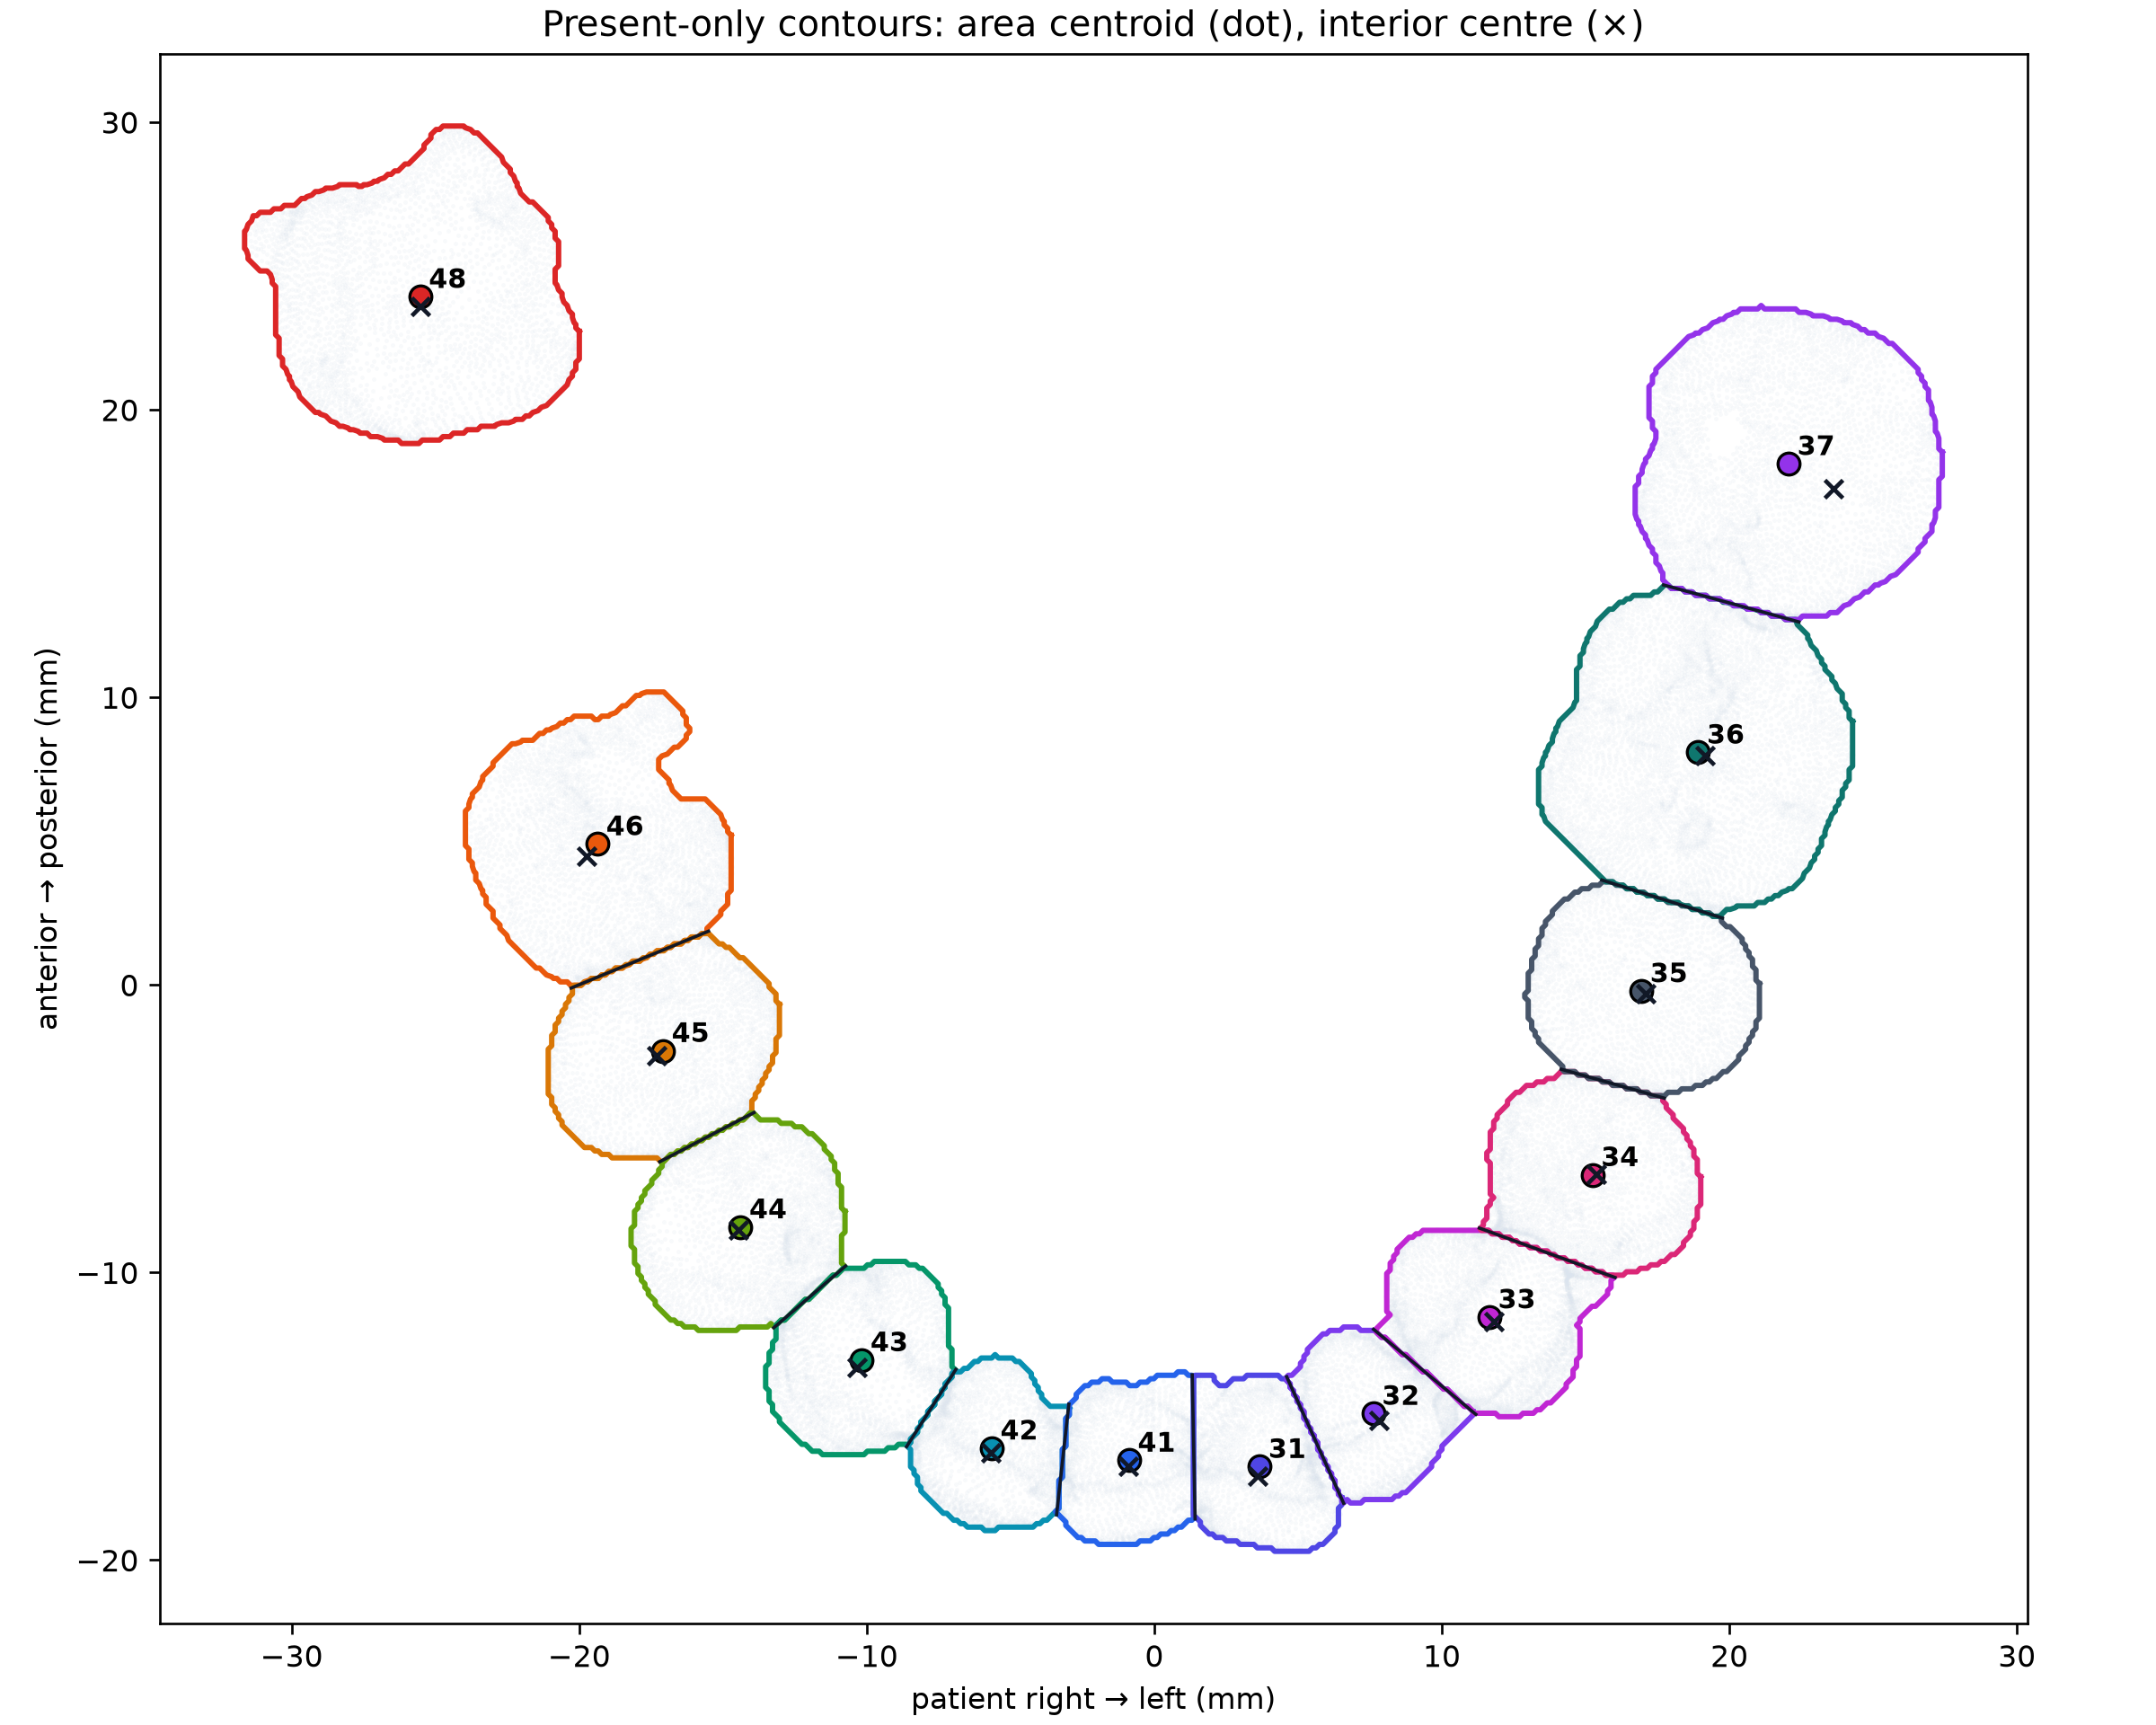
\includegraphics[width=0.82\textwidth]{05_contact_chord_contours.png}
  \caption{批准后的 present-only 接触弦轮廓。圆点是面积质心，叉号是内部参考中心。}
  \label{fig:contact-contours}
\end{figure}

\subsection{沿牙弓排序和 FDI 语义}

各牙中心沿一条有方向的牙弓曲线投影为弧长坐标 $s$。映射报告保存每颗牙的 FDI、
\texttt{arch\_s\_mm}、局部切向、局部外向、牙冠点和导板顶部点。缺失牙和排除牙保留在
FDI 顺序中用于语义推断，但不会创建虚假的“现存牙表面中心”。

\begin{figure}[H]
  \centering
  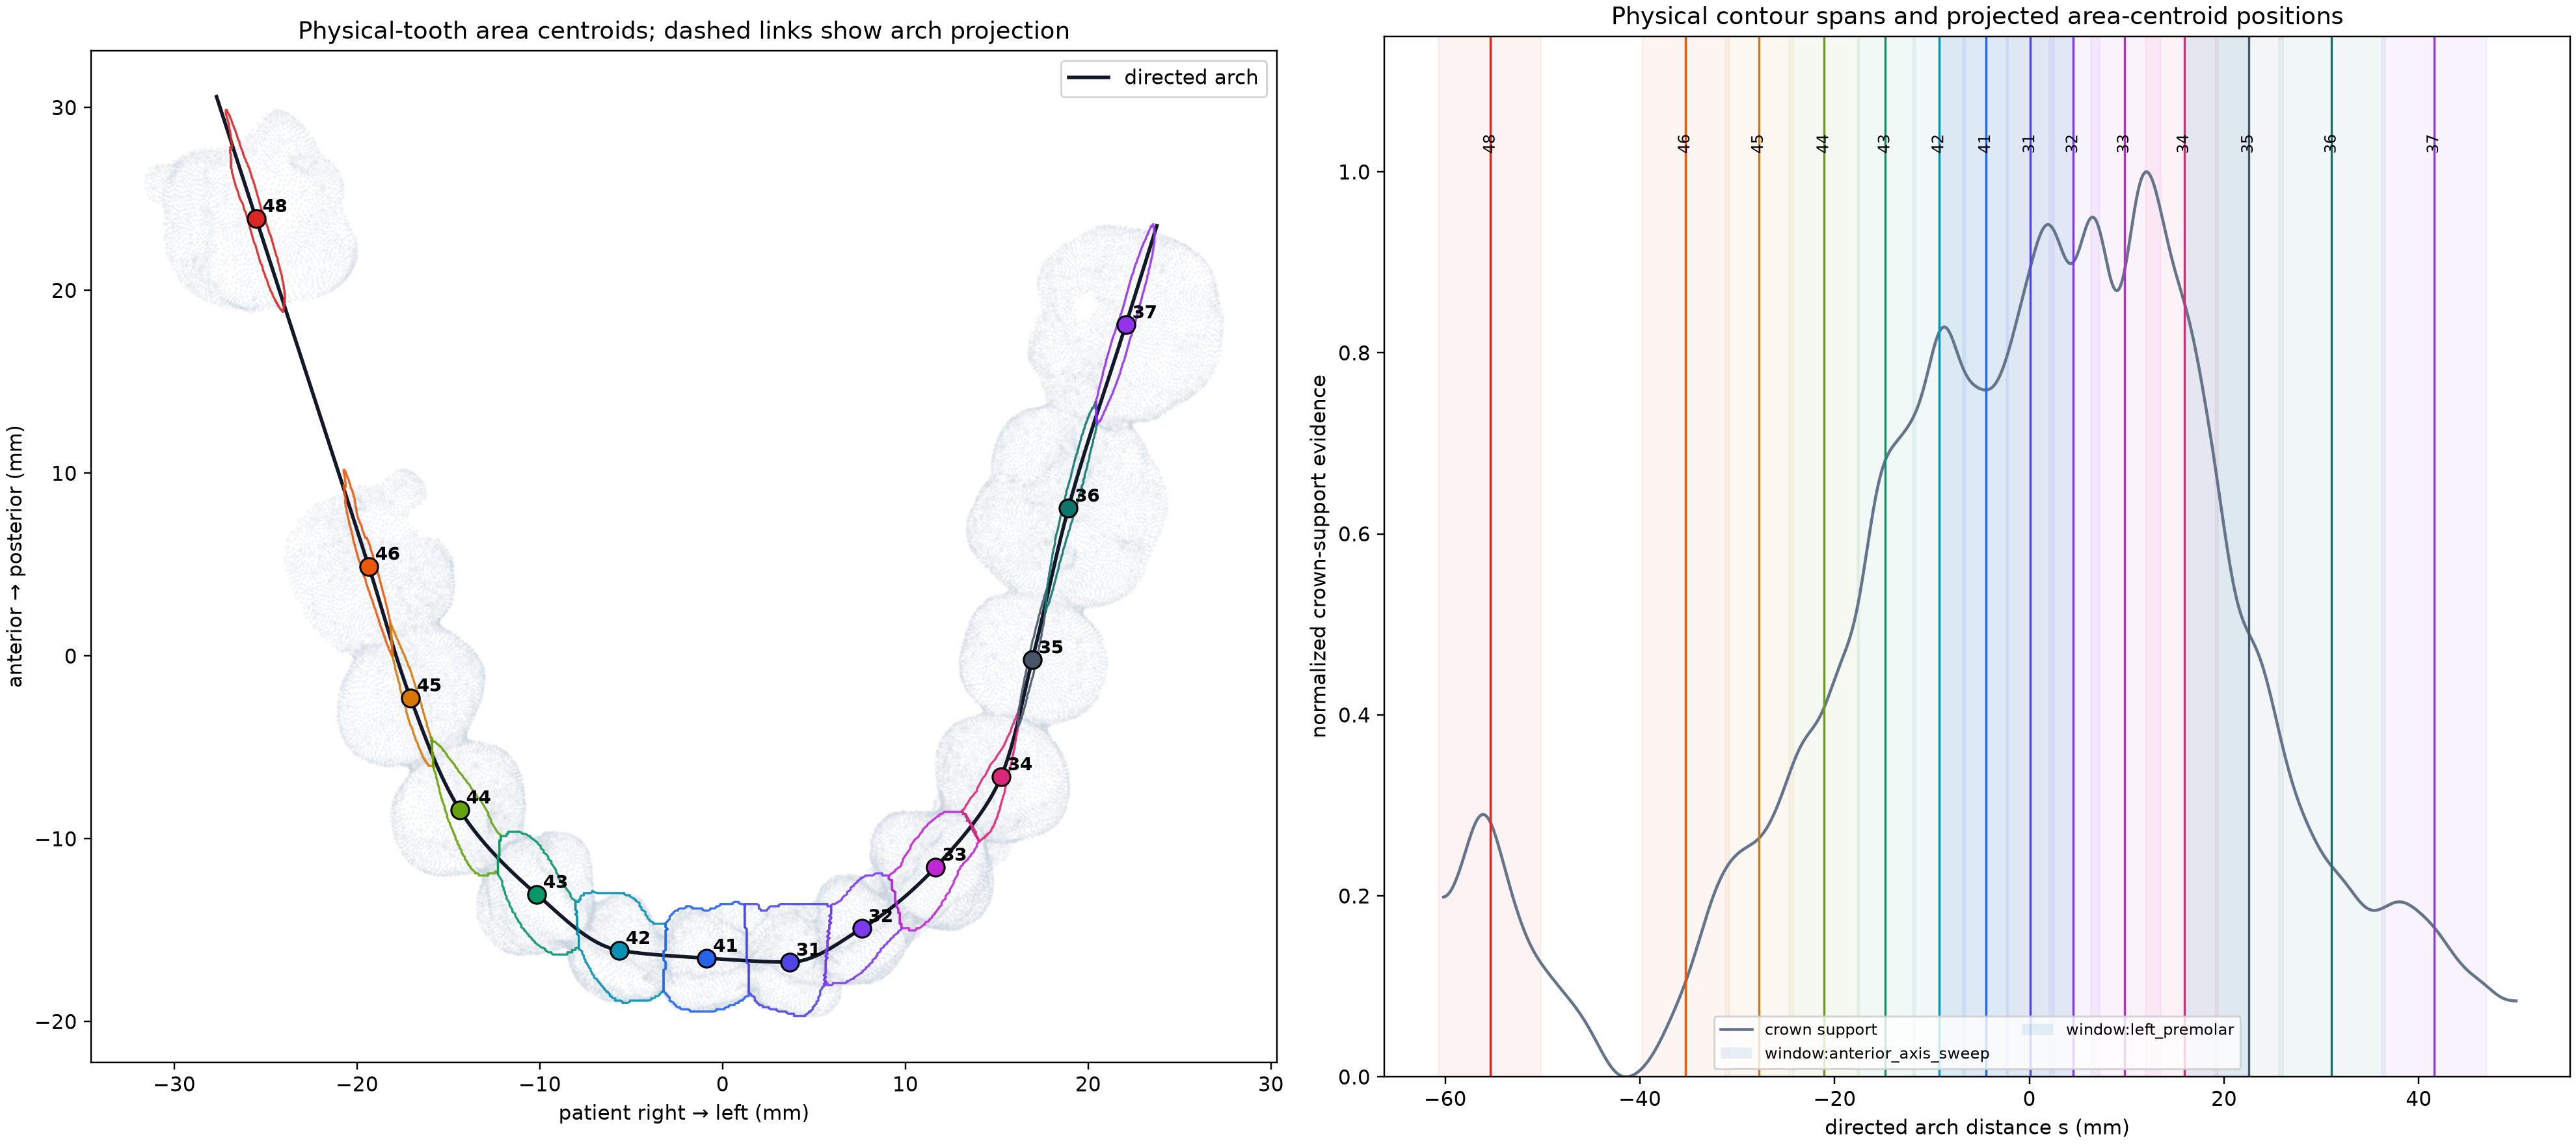
\includegraphics[width=0.98\textwidth]{06_tooth_guide_mapping.png}
  \caption{牙中心、定向牙弓和导板物理覆盖映射。右图把每颗牙的轮廓区间投影到弧长 $s$。}
  \label{fig:tooth-mapping}
\end{figure}

\subsection{左右方向安全门}

自动坐标可能存在左右翻转。若 YAML 没有直接给出确认轴，程序会比较两个候选方向，并在
存在缺失种植牙位时，比较预测缺牙位置到导管手术位的牙弓平面距离。最佳方向通常必须不
超过 15 mm，且比另一方向至少好 3 mm；证据不足即停止。tooth-47 的 YAML 已明确给出
$+X$ 为患者右到左、$+Y$ 为前到后、$+Z$ 为牙合方向，因此报告采用确认轴而非自动二选一。

\subsection{缓存与防陈旧结果}

映射清单记录病例 YAML、牙列、导板和导管参考 STL 的 SHA-256。只有算法版本、输入路径和
摘要全部一致时才允许复用，否则重新执行。生产流程还要求映射状态完整、全部 QA 为真、
上下颌一致、报告中的输入路径与当前配置一致。

\section{步骤三：导孔、操作窗与观察窗}

\subsection{导孔}

每根导管生成一个有限圆柱 cutter。若导管中心为 $\mathbf o$、轴为 $\mathbf a$、轴向范围
为 $[t_{\min},t_{\max}]$、余量为 $m$，则 cutter 两端为
\[
  \mathbf p_0=\mathbf o+(t_{\min}-m)\mathbf a,
  \qquad
  \mathbf p_1=\mathbf o+(t_{\max}+m)\mathbf a.
\]
tooth-47 的轴向余量为 5 mm，规划孔径为 2.10 mm。有限而非无限圆柱能控制差集范围，
又通过上下余量确保穿透融合后的实体。

\subsection{双导管操作窗}

程序在非导管分量中寻找靠近双导管中点、主平面长短比不大于约 1.3 的紧凑圆形操作结构。
操作窗局部标架由两导管平均轴、中心连线投影和二者叉积构成。长边覆盖导管中心距、两侧
导管半径及切向余量；短边覆盖操作特征直径和双侧 bitangent 余量；深度取局部导板厚度与
导管长度的较大者，再加轴向余量。最终 cutter 是带圆角的定向长方体。

\subsection{按 FDI 范围构造轴扫掠观察窗}

观察窗不再使用固定世界坐标下的粗矩形。YAML 指定起止 FDI，牙位映射给出牙弓语义轴和
朝唇颊侧外部的方向。程序沿语义轴布置截面，在每个截面内从牙合方向旋转到外侧方向，形成
约 90° 的扇形扫掠体；自适应射线测量真实导板壁厚，并附加配置的 overcut 以保证穿透。

\begin{figure}[H]
  \centering
  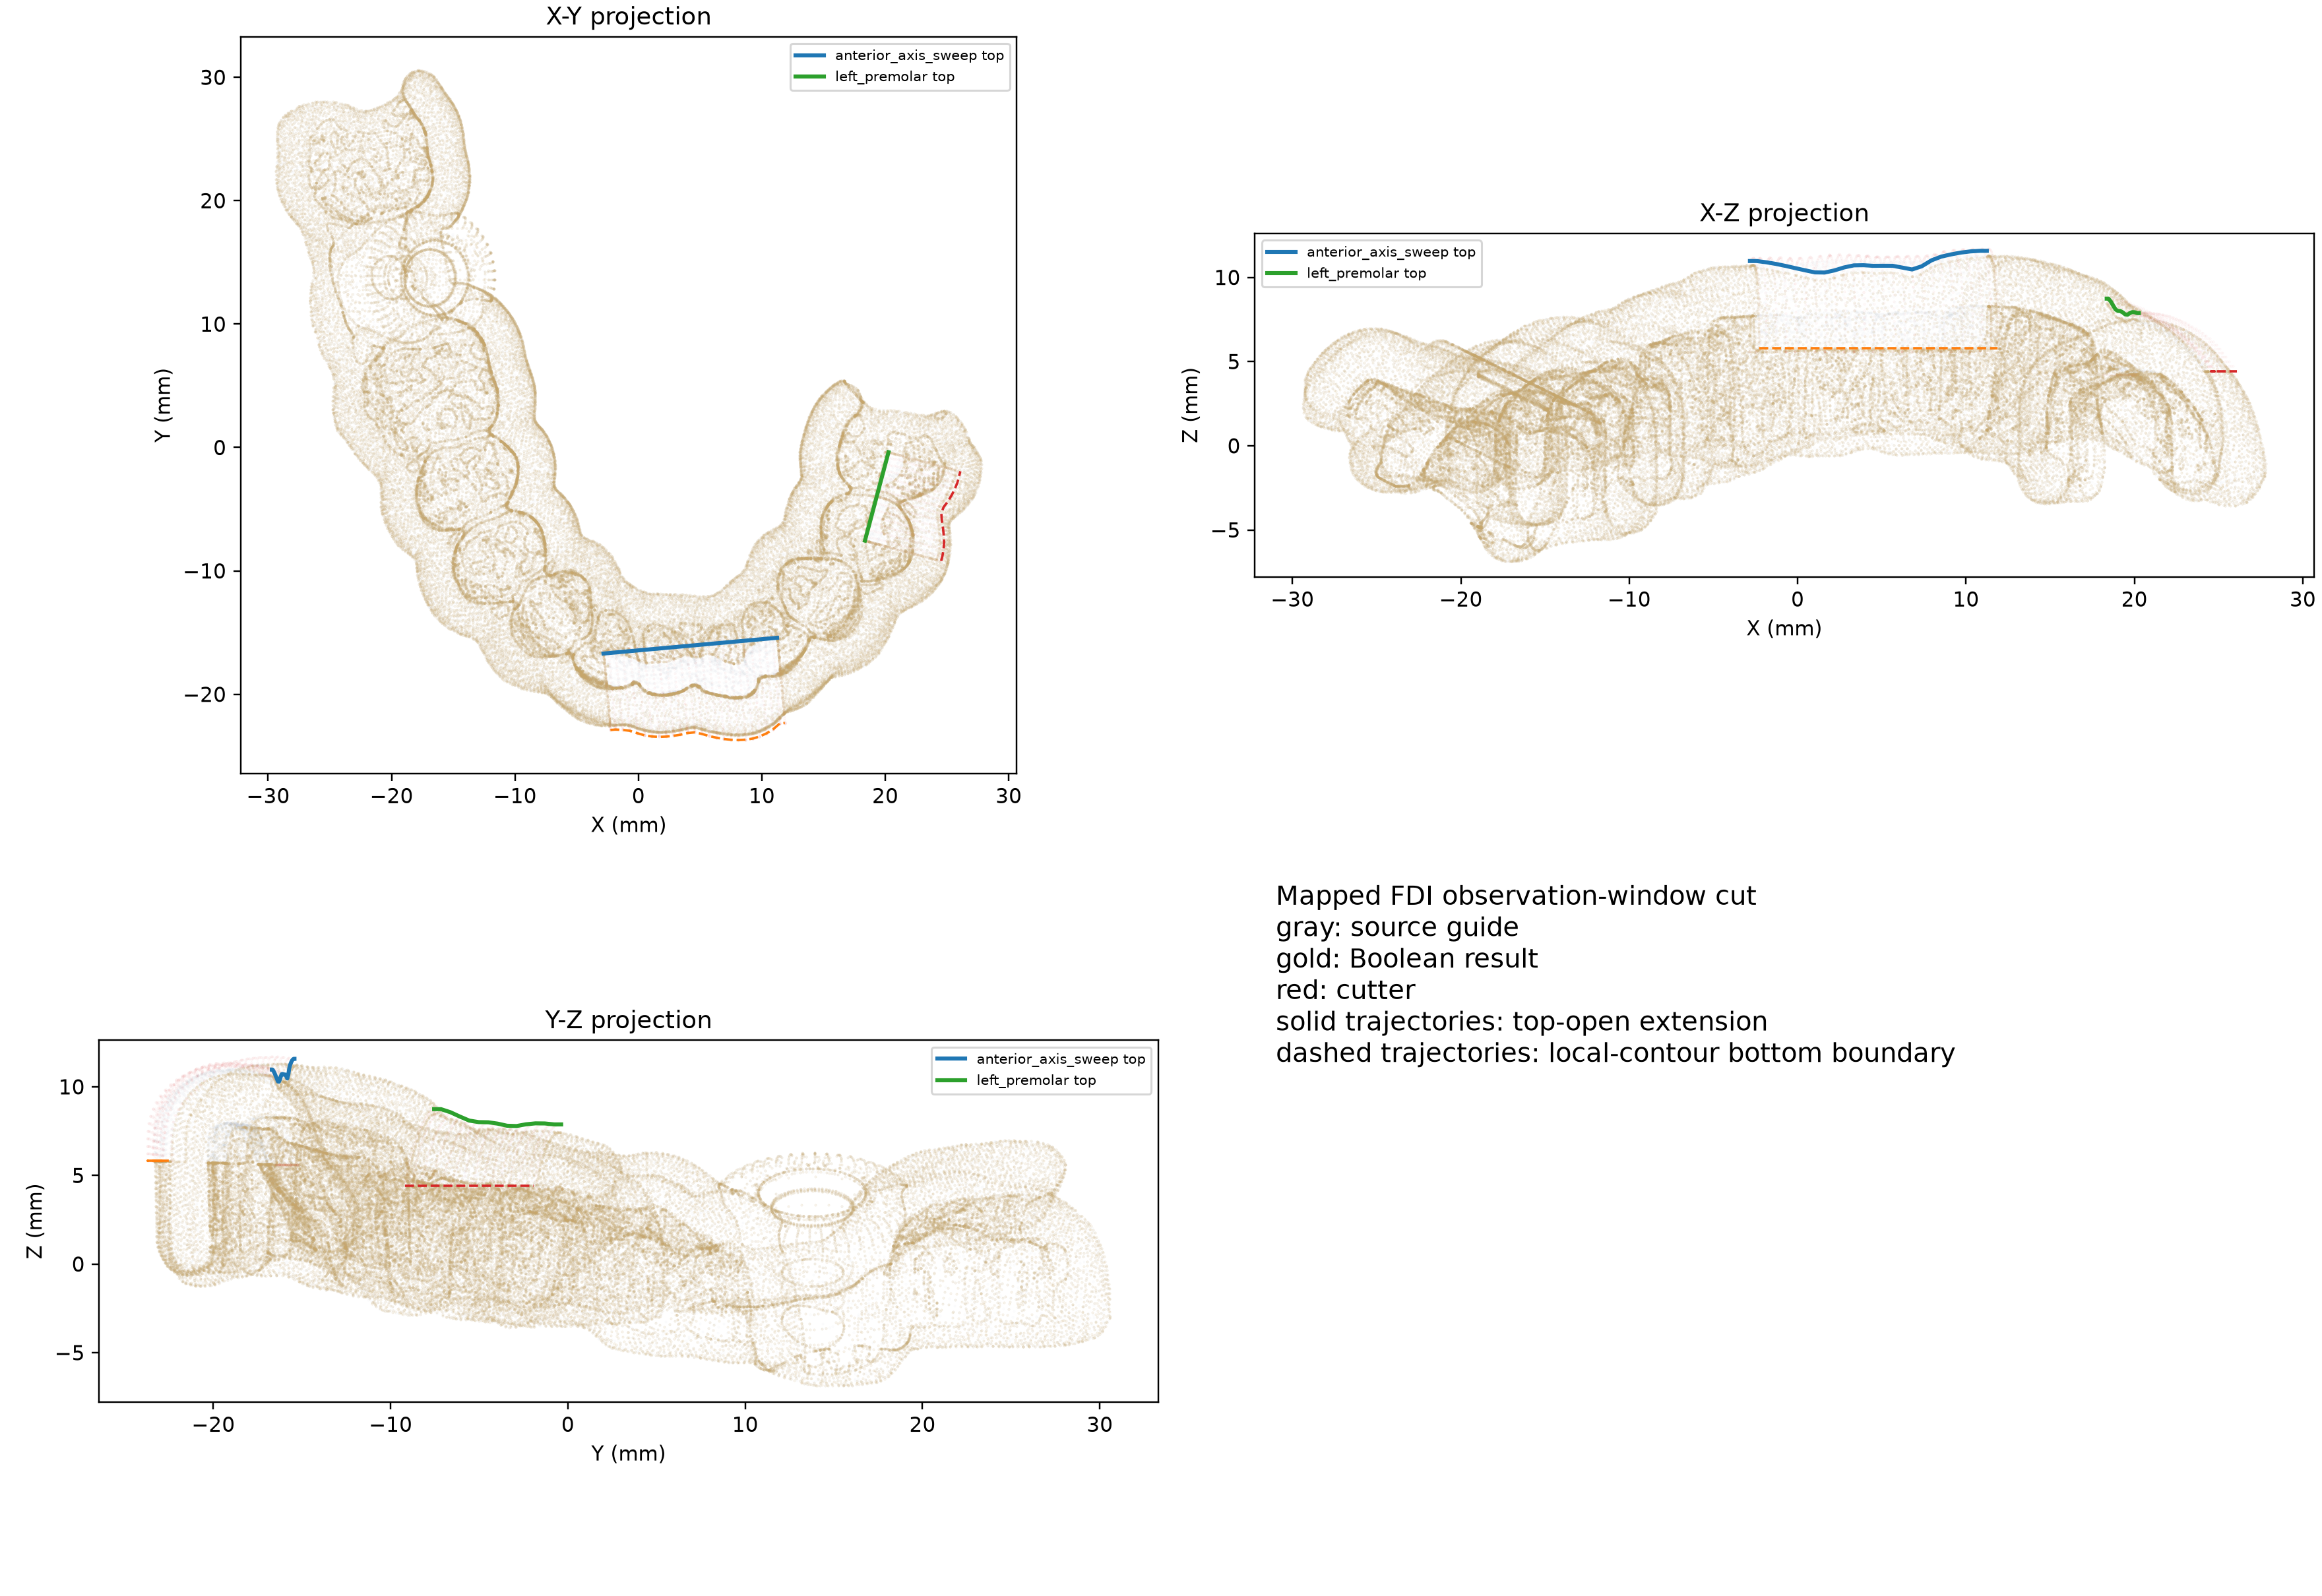
\includegraphics[width=0.96\textwidth]{07_observation_windows.png}
  \caption{tooth-47 两个观察窗的三向投影。蓝线对应 42--32，绿线对应 34--35。}
  \label{fig:observation}
\end{figure}

观察窗生成器检查：组合 cutter 是否为闭合体、是否确实移除材料、语义轴是否连续开放、
是否能看到牙面、是否残留 cutter 重叠、差集体积恒等式是否成立。某些轴行失败时可以按配置
逐级增加局部 drop；修改只写入派生映射，不回写原牙位报告。

\begin{figure}[H]
  \centering
  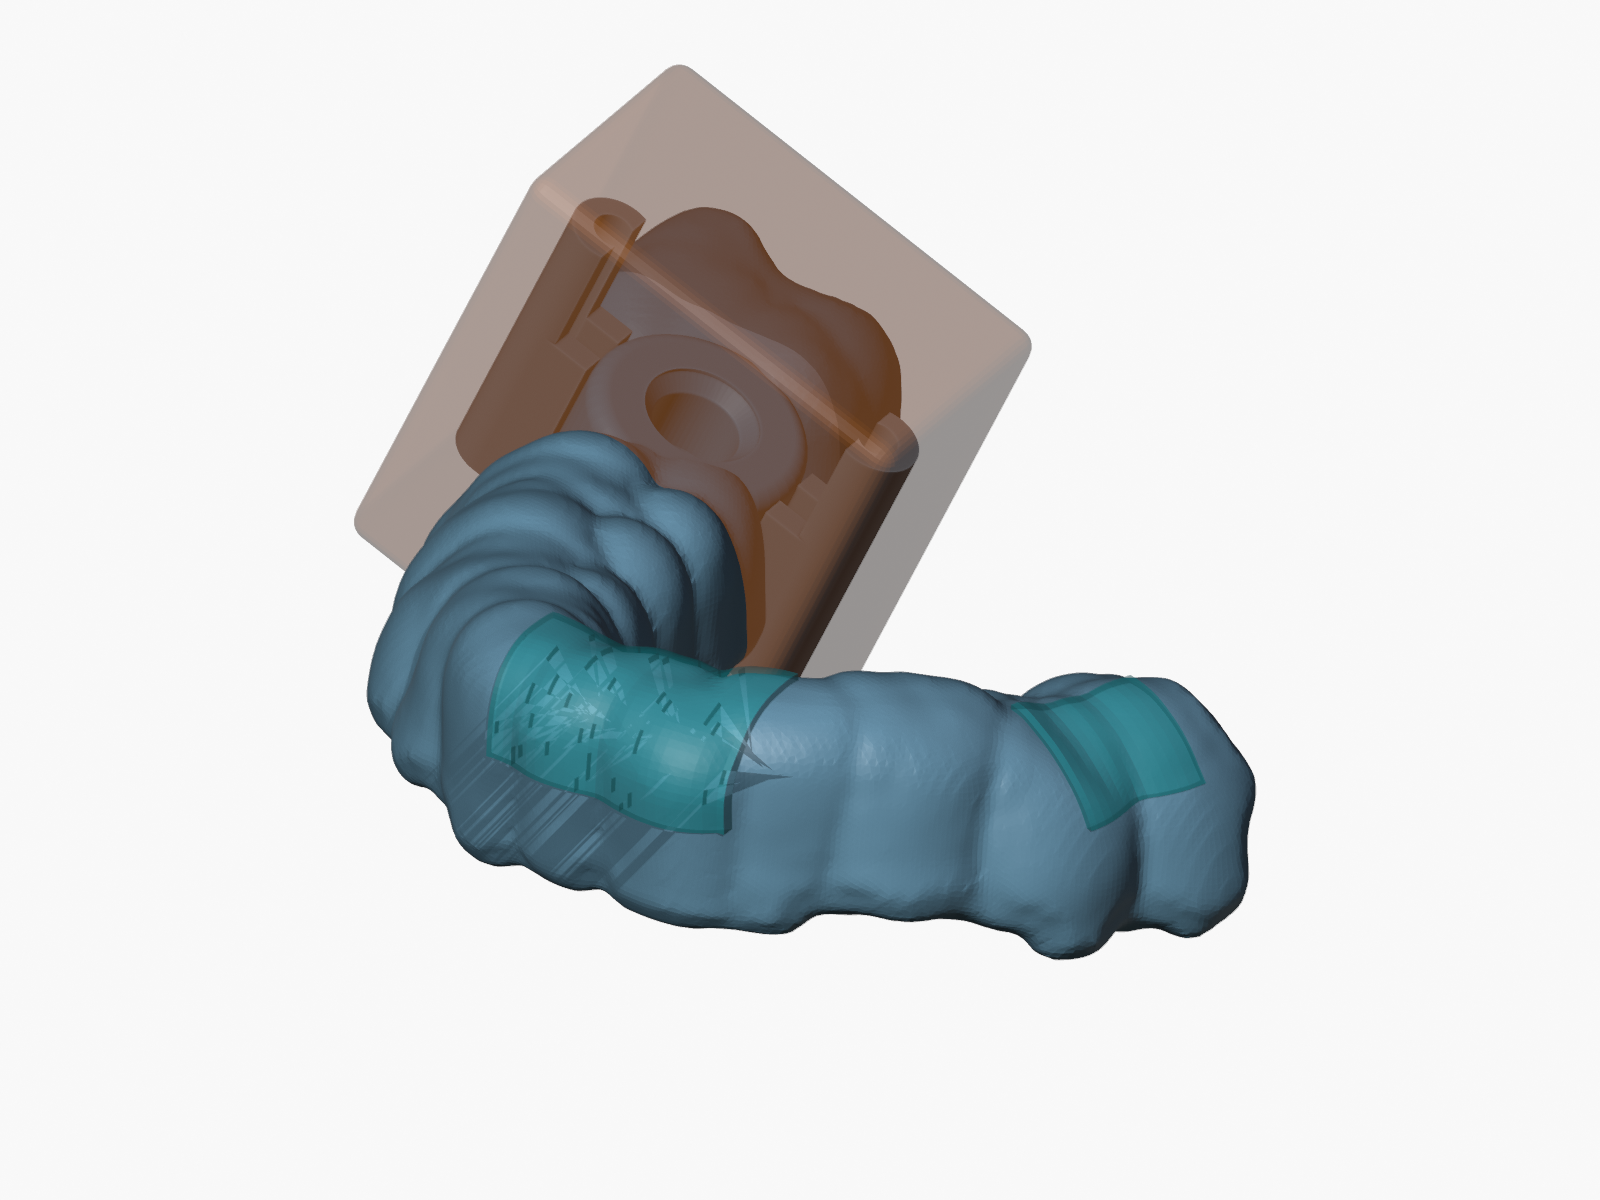
\includegraphics[width=0.78\textwidth]{08_cutouts.png}
  \caption{导孔、操作窗和观察窗 cutter 与导板的空间关系。透明棕色体为操作区，青色体为 FDI 观察窗。}
  \label{fig:cutouts}
\end{figure}

\section{步骤四：导管 Q/P 与导板 A 锚点}

\subsection{导管表面接触点 Q 和中心线点 P}

每根导管在 C 口反方向的稳定外壁母线上选择上下两个截面。高端位置和低端位置分别近似为
\[
  t_{\mathrm{upper}}=t_{\max}-2.0-r,
  \qquad
  t_{\mathrm{lower}}=t_{\min}+1.0+r,
\]
其中 $r$ 是梁半径。由截面中心向外射线命中导管真实外壁得到 Q。若期望梁与导管重叠深度
为 $d$，外壁法向为 $\mathbf n$，中心线点为
\[
  \boxed{\mathbf P=\mathbf Q+(r-d)\mathbf n}.
\]
这一区分很重要：Q 描述实体表面接触，P 描述圆管中心线。直接把中心线放在 Q 上只能得到
半径级接触，不能表达受控预埋。

\subsection{牙位参考点 T 与旋转射线}

导板端不再按整条切面轨迹的 20\%/80\% 弧长取点。对单牙中心或双牙中点站位，先取附近牙冠
最高点 $\mathbf H$，再沿正牙合方向向内下移 2 mm：
\[
  \mathbf T=\mathbf H-2\,\mathbf e_{\mathrm{occ}}.
\]
单牙站位使用最近且被导板覆盖的邻牙建立旋转面；双牙站位使用两牙中心连线。旋转射线为
\[
  \mathbf d(\theta)=
  \cos\theta\,\mathbf e_{\mathrm{occ}}+
  \sin\theta\,\mathbf e_{\mathrm{side}},
\]
其中 $\mathbf e_{\mathrm{side}}$ 的符号由该牙位的 \texttt{local\_outward} 决定，因此 U 侧和
背 U 侧不是屏幕左/右。主梁常用 U 侧 70°、背 U 侧 90°，但每个锚点都可独立配置。

\subsection{为什么选择“外壁出口”}

射线与薄壳导板可能产生入口、内壁、外壁和重复三角交点。程序把射线参数距离相差小于
0.02 mm 的交点聚类，再检查命中面法向与射线方向的点积；首个法向朝射线方向且点积不小于
0.05 的交点才被视为外壁出口 A。这样可以避免把内壁入口误当作梁端。

\subsection{独立端点与导管配对}

每个端部配置一个 U 侧和一个背 U 侧锚点。程序比较直接配对与反向配对的总距离，使每根
导管从两个端部各获得一个锚点。这保证每根梁都跨越两个导板区域，而不是让一根导管只连接
到同一局部区域。

\begin{figure}[H]
  \centering
  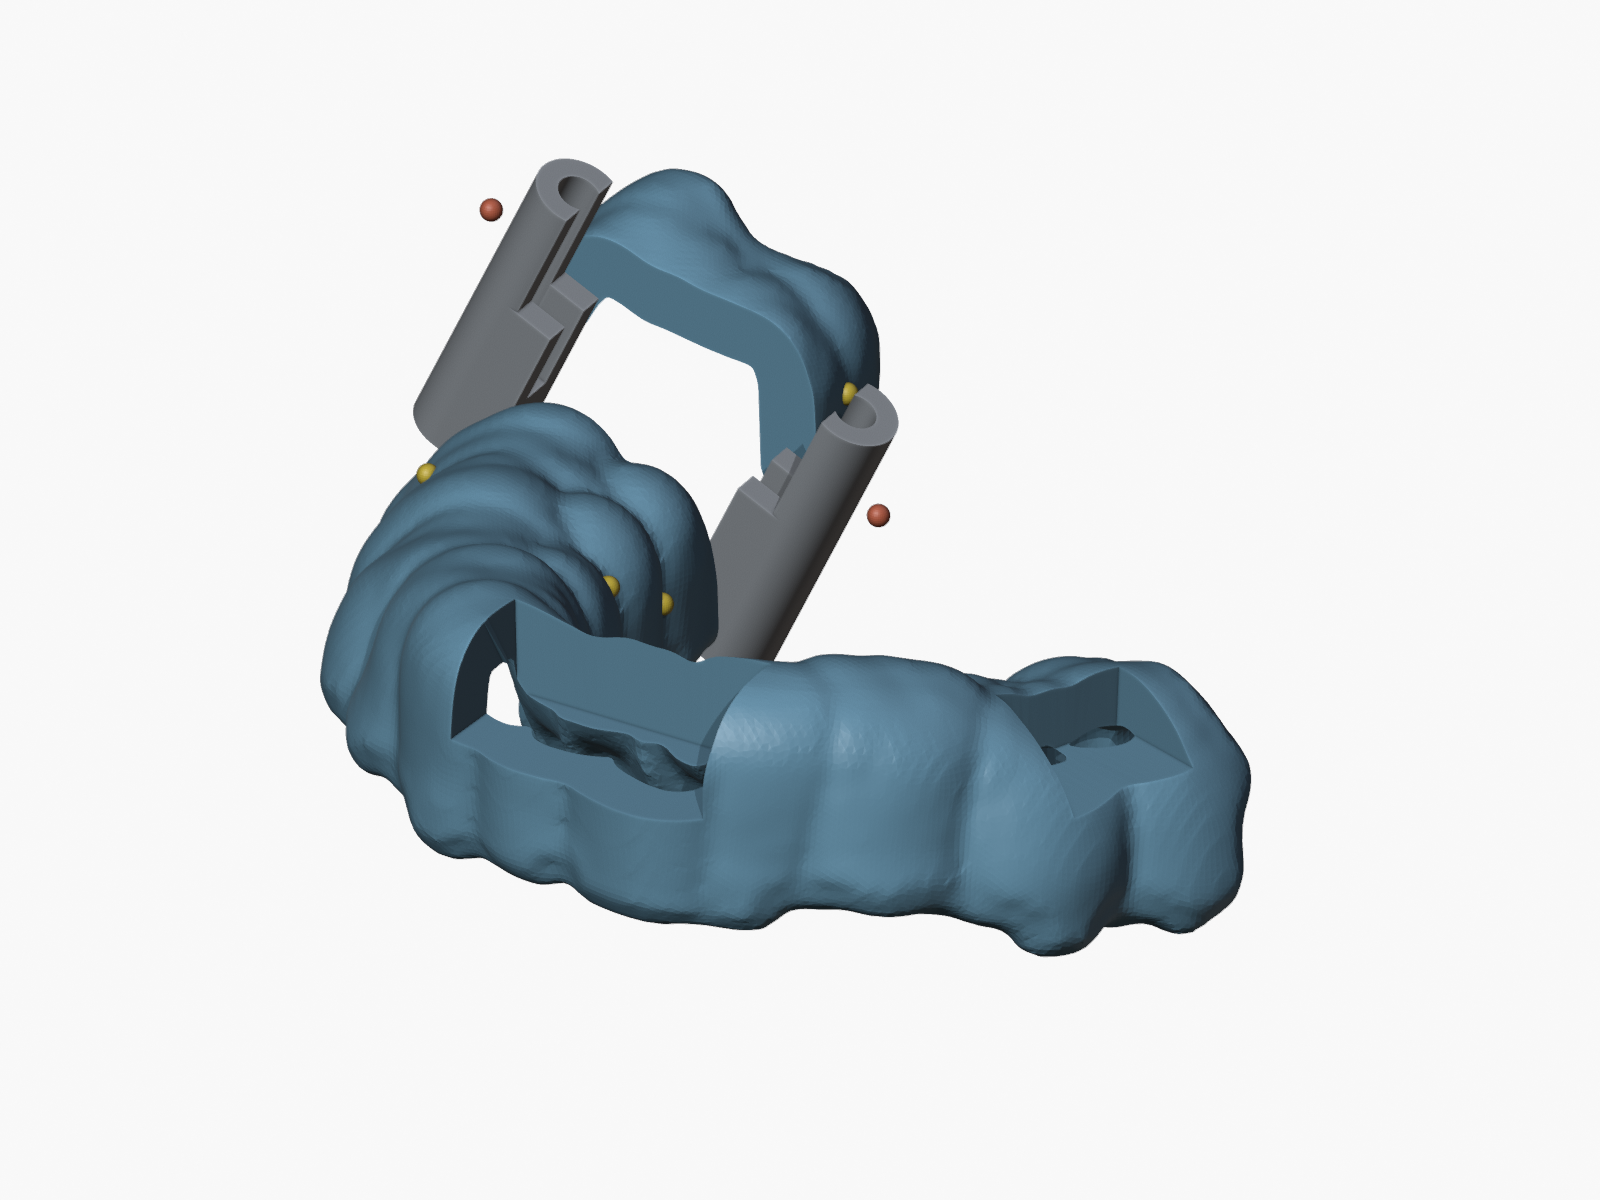
\includegraphics[width=0.82\textwidth]{09_link_points.png}
  \caption{tooth-47 锚点可视化。黄色标记为导管侧 Q/P 相关点，棕色标记为导板端锚点。}
  \label{fig:anchors}
\end{figure}

\section{步骤五与六：四根主梁、Y 型按压梁和实体扫掠}

\subsection{主梁拓扑}

每根导管生成高、低两根连续梁，均从一个导板端出发，经导管 P 点到另一个导板端。因此一个
种植位的两根导管共四根主梁。高梁直接经过高端 P；低梁先构造外层代理曲线，再只在 P 附近
局部下潜，降低大范围弯折和孔道侵入风险。

\subsection{五次 Hermite 曲线}

每段曲线采用端点二阶导数为零的五次 Hermite 基函数：
\begin{align*}
  \mathbf C(u)=&\;h_0(u)\mathbf p_0+h_1(u)\mathbf m_0
  +h_2(u)\mathbf p_1+h_3(u)\mathbf m_1,\quad u\in[0,1],\\
  h_0=&1-10u^3+15u^4-6u^5,\\
  h_1=&u-6u^3+8u^4-3u^5,\\
  h_2=&10u^3-15u^4+6u^5,\\
  h_3=&-4u^3+7u^4-3u^5.
\end{align*}
两段在导管 P 共享一阶导数，避免折线式尖角。端点切向先投影到相应表面切平面，再按端点
距离和张力系数缩放。中心线按约 0.30 mm 间距离散，且每段至少 17 个奇数采样点。

\subsection{低梁局部下潜}

低梁的外层代理接触点位于外壁 Q 附近。程序在代理曲线两侧约 5 mm 弧长处选择拼接点，
左拼接继承左侧自然切向，右拼接继承右侧自然切向，只有深埋 P 使用左右拼接点连线方向。
这一设计修复了“整段共用一个方向”导致的两侧切向不连续。

\subsection{Y 型按压梁}

当前支持三种模式：

\begin{itemize}
  \item \texttt{inner\_sleeve\_upper\_y}：一个锚点在内侧导管高端，两个在导板；
  \item \texttt{three\_tooth\_anchors\_y}：三个锚点全部由牙位射线落在导板；
  \item \texttt{terminal\_u\_extension\_anchor\_y}：一个锚点落在末端 U 梁，两个在导板。
\end{itemize}

三牙位模式取三个中心线锚点的算术中心，并沿病例确认的牙合轴抬高默认 2 mm。程序检查
三锚点展开面积、最短边和汇合点处最小臂角（默认至少 25°），避免近乎共线的“假 Y 型”。
末端 U 梁模式则在允许中心线上最大化到两个导板锚点的较小距离，即 maximin 选点。

\subsection{平行输运圆管扫掠}

直接使用 Frenet 标架会在曲率接近零或反曲点处突然翻转。项目先估计离散切向，再用相邻
切向的叉积确定最小旋转轴，通过 Rodrigues 旋转把前一截面法向输运到下一截面。随后每个
采样点构造 64 边圆环并连接相邻圆环，封闭首尾端盖。

\subsection{根部渐粗、球头与贴合脚}

梁在导板端最后约 3 mm 通过 smoothstep 从标准半径渐粗到约 1.08 倍；同一唯一导板端再增加
根部球和曲面贴合椭圆脚。贴合脚向导板内预埋 0.25 mm，并按局部表面投影。若完整足印投影
距离超过 1.56 mm，程序逐步缩小足印，最低到 77\%；仍超限时只发出警告并继续生成。

\begin{figure}[H]
  \centering
  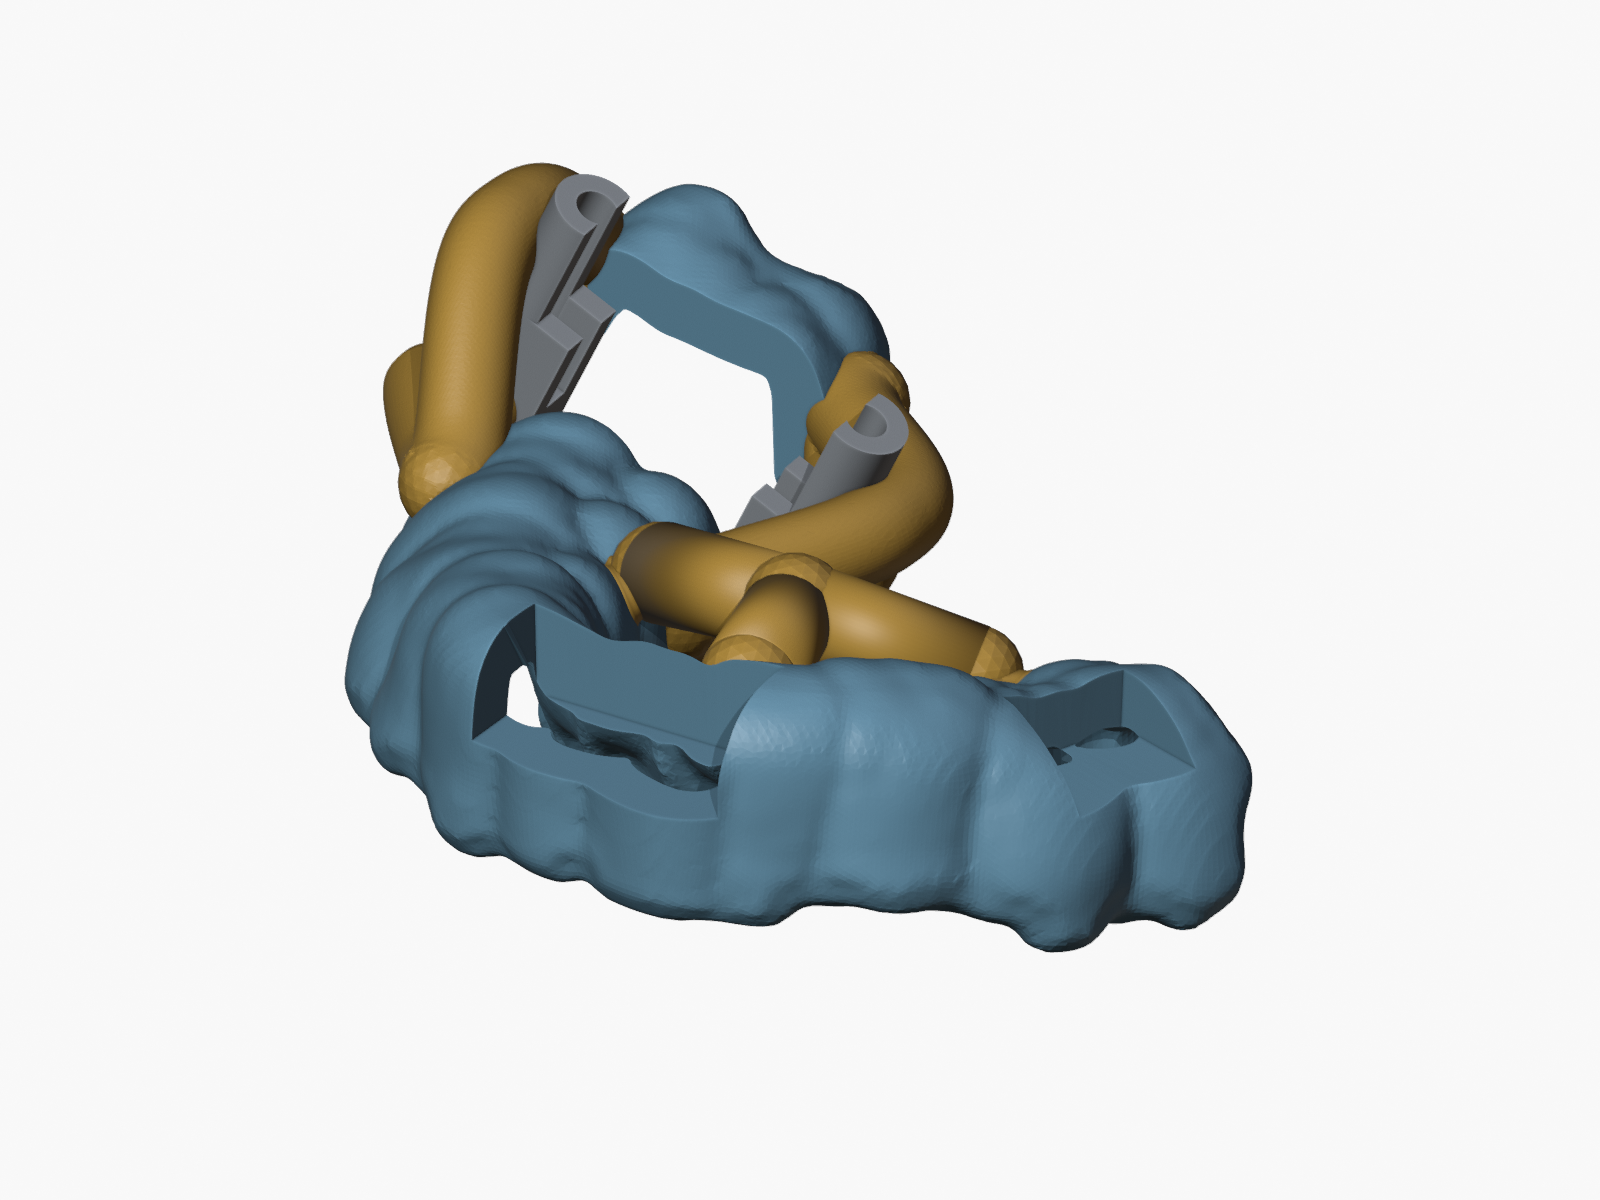
\includegraphics[width=0.84\textwidth]{10_connectors.png}
  \caption{tooth-47 主梁、Y 梁、根部强化与导管的装配预览。金色为新增梁架。}
  \label{fig:connectors}
\end{figure}

\section{特殊病例拓扑}

这些结构不是 tooth-47 的主线，但属于“整个项目”必须交接的能力。

\begin{description}
  \item[两分量断裂导板跨接] 要求导板恰好有两个主要分量，在两个牙位站位分别求 U/背 U
  锚点，使同侧锚点跨越不同分量，生成两根直线跨接梁。
  \item[末端 U 型延伸] 用于末端牙存在但导板覆盖过短。程序从参考邻牙指向末端牙确定远中
  方向，优先依据末端牙闭合轮廓外扩“梁半径 + 牙体净距 + 安全余量”，构造切向连续 U 梁。
  \item[远中公共节点] 用于末端牙缺失且远中无导板。以两根末端导管低端 P 中点 $\mathbf B$
  为基准，沿同时垂直于导管连线和公共轴线的远中方向移动两个平均外径：
  $\mathbf G=\mathbf B+2D\mathbf e_{\mathrm{distal}}$，四根主梁共享 G。
  \item[相邻双种植位连续路径] U 侧和背 U 侧各生成一条跨两个种植位的连续路径，上下两层
  各执行一次，仍得到四根主梁。
\end{description}

末端 U 型延伸与远中公共节点在当前配置中互斥，因为二者代表“有末端牙可绕行”和“末端缺牙
自由闭合”两种不同策略。

\section{牙列净距、体素融合与精确布尔}

\subsection{牙列保护裁剪}

主梁、Y 梁和根部强化先合并为梁架，再用牙列网格作为 cutter，并附加配置的
\texttt{connector\_dental\_clearance\_mm}。这样导板端可以直接以表面 A 点作为中心线端点，
让梁充分进入导板；侵入牙列的部分由差集统一清除。

\subsection{为什么使用体素融合}

多个圆管、球、贴合脚、导管和扫描导板往往只有局部重叠，直接精确并集容易因共面、薄片和
非流形输入失败。\texttt{voxel\_union()} 复制对象、拼接后按 0.2 mm 体素重网格，得到一致
封闭壳体。其代价是细节误差约为体素量级，薄壁、窄孔和尖锐边会被平滑或回缩。

\subsection{差集后端与修复}

初始导板预览使用 Blender 布尔求解器按 EXACT、MANIFOLD、FLOAT 回退；关键的复切和手机
避让使用 manifold3d 连续差集。cutter 默认做 0.02 mm Minkowski 外扩并以 0.005 mm 简化，
减少共面残留。多个 cutter 在同一 manifold 会话中连续扣除，避免中间结果反复序列化为
浮点网格。

如果 STL 序列化产生亚微米重合点或不超过 0.02 mm 的短坏边，代码允许局部焊接或折叠；
修复后必须重新加载并确认为单一封闭体。超过阈值则失败，避免以大尺度自动修复掩盖真实
几何错误。

\section{手机运动包络避让}

程序读取手机 STL 的最大面积连通分量，从止挡报告取得配对止挡面中心和公共轴。两中心中点
作为枢轴 $\mathbf c$，在 $[-5^\circ,5^\circ]$ 内采样 41 个姿态。对任意手机点
$\mathbf p$，第 $k$ 个姿态为
\[
  \mathbf p_k=\mathbf c+\mathbf R(\mathbf a,\theta_k)(\mathbf p-\mathbf c).
\]
所有姿态精确并集成封闭包络，再从最终结构做差集。当前不模拟轴向下压；也不保护进入包络
的梁，因此避让后梁可能被切断，必须重新检查连续性。

\section{两种最终布尔顺序}

\begin{figure}[H]
\centering
\begin{tikzpicture}[
  node distance=5mm,
  box/.style={draw=TGBlue,rounded corners,fill=TGLightBlue,text width=6.2cm,
    minimum height=8mm,align=center,font=\small},
  arrow/.style={-{Latex[length=2mm]},thick,color=TGBlue}
]
  \node[box] (g1) {generated：先切原导板};
  \node[box,below=of g1] (g2) {导板 + 重建导管 + 梁架体素融合};
  \node[box,below=of g2] (g3) {复切导孔与观察窗};
  \node[box,below=of g3] (g4) {手机包络差集、最大连通体、修复导出};
  \draw[arrow] (g1)--(g2);\draw[arrow] (g2)--(g3);\draw[arrow] (g3)--(g4);

  \node[box,right=15mm of g1] (i1) {input：先切原导板};
  \node[box,below=of i1] (i2) {导板 + 梁架体素融合（暂不含导管）};
  \node[box,below=of i2] (i3) {基础体复切孔/窗并做手机差集};
  \node[box,below=of i3] (i4) {最后融合受保护输入导管，仅清亚体素碎片};
  \draw[arrow] (i1)--(i2);\draw[arrow] (i2)--(i3);\draw[arrow] (i3)--(i4);
\end{tikzpicture}
\caption{generated 与 input 模式必须采用不同的复切顺序。}
\label{fig:boolean-order}
\end{figure}

\section{导出、过程图与独立验证}

生成器输出最终 STL、四个标准视图以及输入、导管、锚点、梁架和切口过程图。验证器随后
检查：边界边、非流形边、重复三角形、连通体；导管表面保留率；主梁中心线包覆率；根部球
和贴合脚；Y 梁三臂；导孔多截面多半径探针；观察窗脊线净空。关键默认阈值包括导管保留率
0.90、梁中心线保留率 0.95、观察窗脊线净距 0.20 mm。

验证器的意义是检测“规划看起来正确、但最终布尔破坏了结构”的情况；它不是临床适配验证，
也没有替代实体试戴、打印工艺补偿和医疗审核。


\chapter{tooth-47 案例复盘}

\section{病例定位}

规范病例目录为 \projectpath{data/cases/single/tooth-47}，来源是旧数据中的“初始案例”，
现被定义为黄金回归病例。它是下颌病例，FDI 顺序覆盖 48 到 37；47 缺失，38 排除，实际
识别到 14 颗现存牙。牙合方向为 $+Z$，患者右到左为 $+X$，前到后为 $+Y$。

\begin{table}[H]
\centering
\begin{tabularx}{\textwidth}{p{0.29\textwidth}X}
  \toprule
  项目 & tooth-47 当前配置\\
  \midrule
  病例角色 & 单颗缺牙黄金回归；\texttt{validated\_current\_workflow}\\
  导管实体模式 & \texttt{input}，直接采用识别出的输入导管\\
  现存/缺失/排除 & 14 颗现存牙；缺失 47；排除 38\\
  主梁锚点站位 & 48，以及 46/45 双牙中点；U 侧 70°、背 U 侧 90°\\
  Y 梁模式 & \texttt{three\_tooth\_anchors\_y}\\
  Y 梁三个站位 & 45/44（75°）、31/32（45°）、34/35（75°）\\
  观察窗 & 42--32 前牙窗；34--35 左前磨牙窗\\
  观察窗几何 & 轴向下移 0.5 mm，扫掠 90°，高度 5 mm，顶部开放\\
  梁直径 / 体素尺寸 & 4.60 mm / 0.20 mm\\
  手机运动 & 当前深度，$-5^\circ$ 到 $+5^\circ$，41 姿态\\
  \bottomrule
\end{tabularx}
\caption{tooth-47 的主要病例和工程参数。}
\end{table}

\section{牙位与牙弓映射结果}

映射报告状态为 \texttt{tooth\_guide\_mapping\_complete}，全部 16 项 QA 为真。最终牙中心
来自批准接触弦轮廓的均匀面积质心；有向牙弓由这些质心的参数化 PCHIP 曲线及末端轮廓支撑
扩展构成。现存牙平均支持证据为 0.5334，缺失槽位平均支持为 0.0019，说明缺失 47 的语义
与实际表面支持有明显区分。

由于病例 YAML 已确认三条坐标轴，当前映射没有启用“缺失牙到手术位”二选一安全门；这并非
安全门失效，而是人工确认轴优先于自动候选比较。

\section{两个观察窗的实际结果}

\begin{table}[H]
\centering
\small
\begin{tabularx}{\textwidth}{lrrrrX}
  \toprule
  窗口 & 轴长/mm & 轴截面 & cutter 体积/mm$^3$ & 最小轴净空/mm & 牙面可见性\\
  \midrule
  42--32 前牙窗 & 13.323 & 24 & 519.062 & 0.2023 & 24/24 轴行可见\\
  34--35 前磨牙窗 & 6.615 & 13 & 116.842 & 0.1992 & 12/13 轴行可见\\
  \bottomrule
\end{tabularx}
\caption{tooth-47 观察窗过程报告中的关键数据。}
\end{table}

两个窗的连续清晰走廊比例均为 1.0。前牙窗实际测得壁厚约 3.00--7.28 mm，中位数 3.73 mm；
前磨牙窗约 2.96--5.30 mm，中位数 3.45 mm。源导板体积为 $6364.52\,\mathrm{mm^3}$，切窗后
为 $5881.56\,\mathrm{mm^3}$，实际移除 $482.96\,\mathrm{mm^3}$。布尔体积恒等误差仅
$0.00167\,\mathrm{mm^3}$，残余 cutter 重叠约 $4.81\times10^{-6}\,\mathrm{mm^3}$。

初始 0.5 mm 轴下移已经通过全部 QA，因此没有应用 1/2/3 mm 的局部回退。这里必须以
tooth-47 实际 JSON/报告为准：项目部分文档仍写着 0.2 mm 和 0.5/1/2 mm 回退，属于文档与
当前病例参数的漂移。

\section{连接结构与结果外观}

图 \ref{fig:connectors} 已展示融合前新增梁架。tooth-47 的四根主梁均为 4.60 mm 直径，并在
导板端采用 1.08 倍根部半径、3 mm 过渡、球头和曲面贴合脚。Y 梁三个端点全部来自牙位 U 侧
射线，汇合点沿 $+Z$ 抬高 2 mm。

\begin{figure}[H]
  \centering
  \begin{subfigure}[t]{0.48\textwidth}
    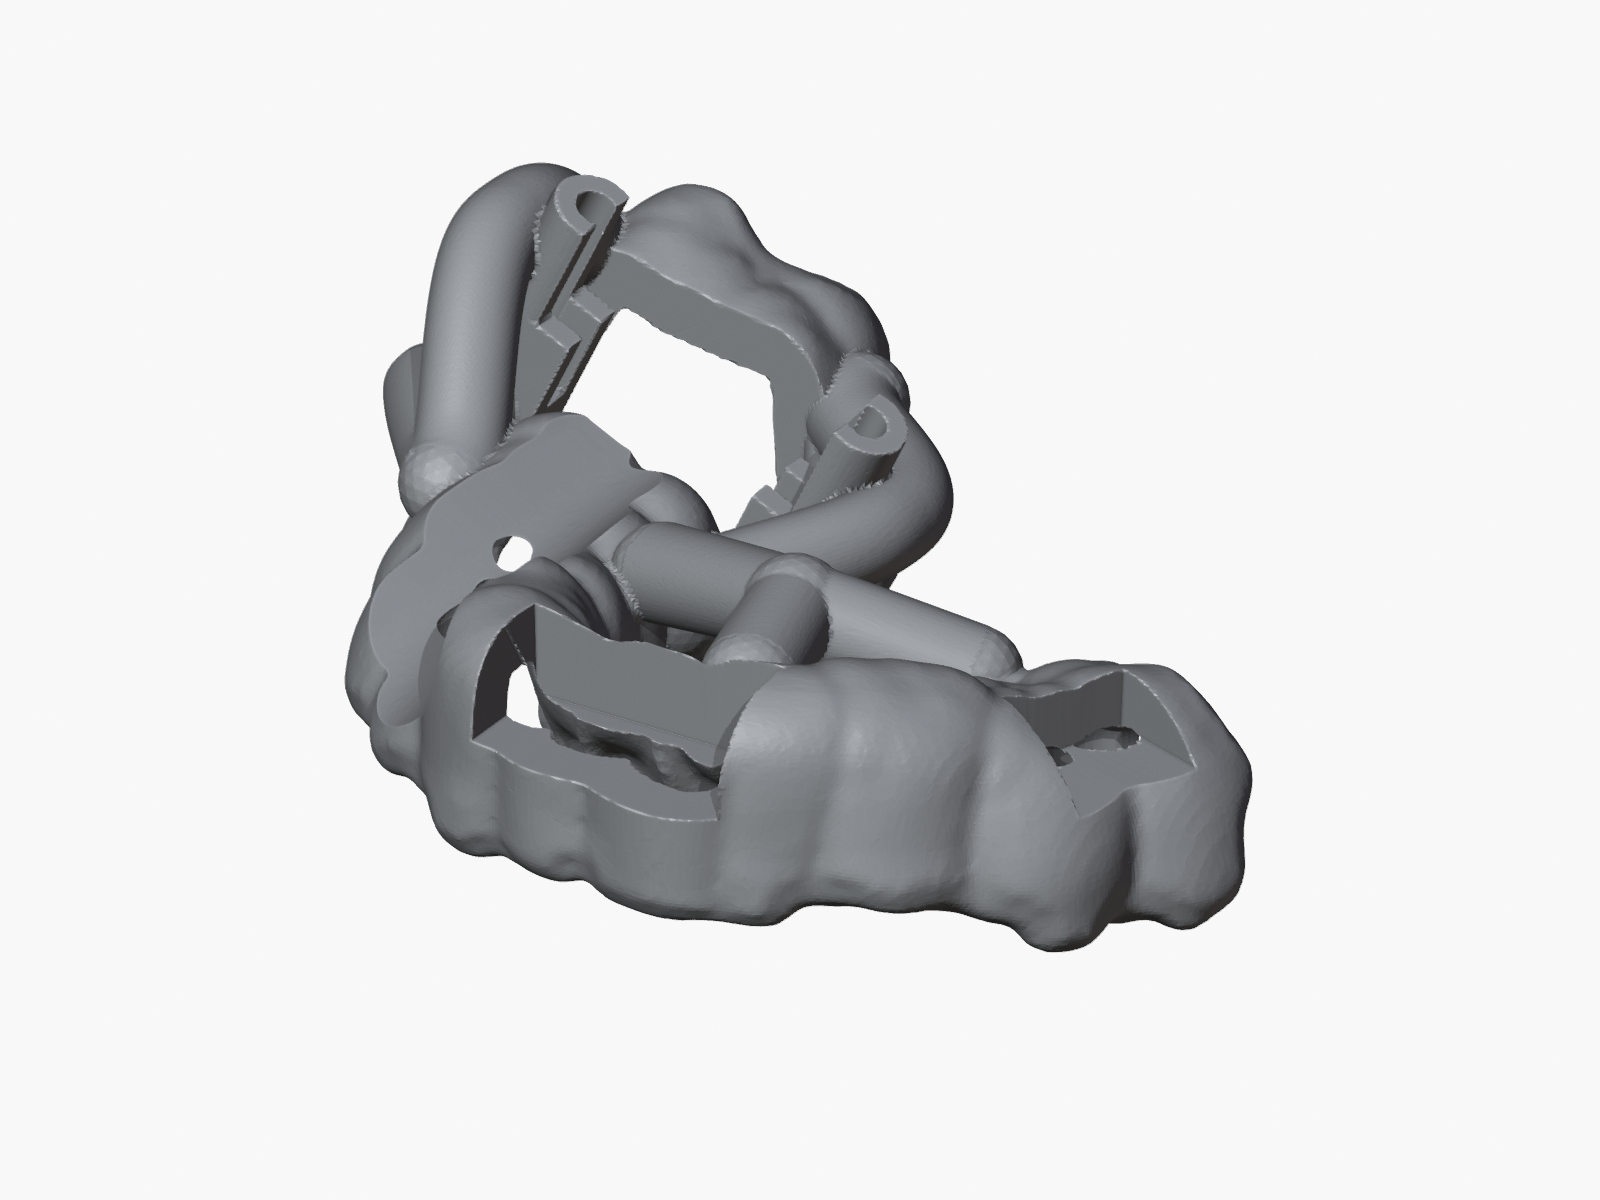
\includegraphics[width=\linewidth]{11_final_iso.png}
    \caption{等轴视图}
  \end{subfigure}\hfill
  \begin{subfigure}[t]{0.48\textwidth}
    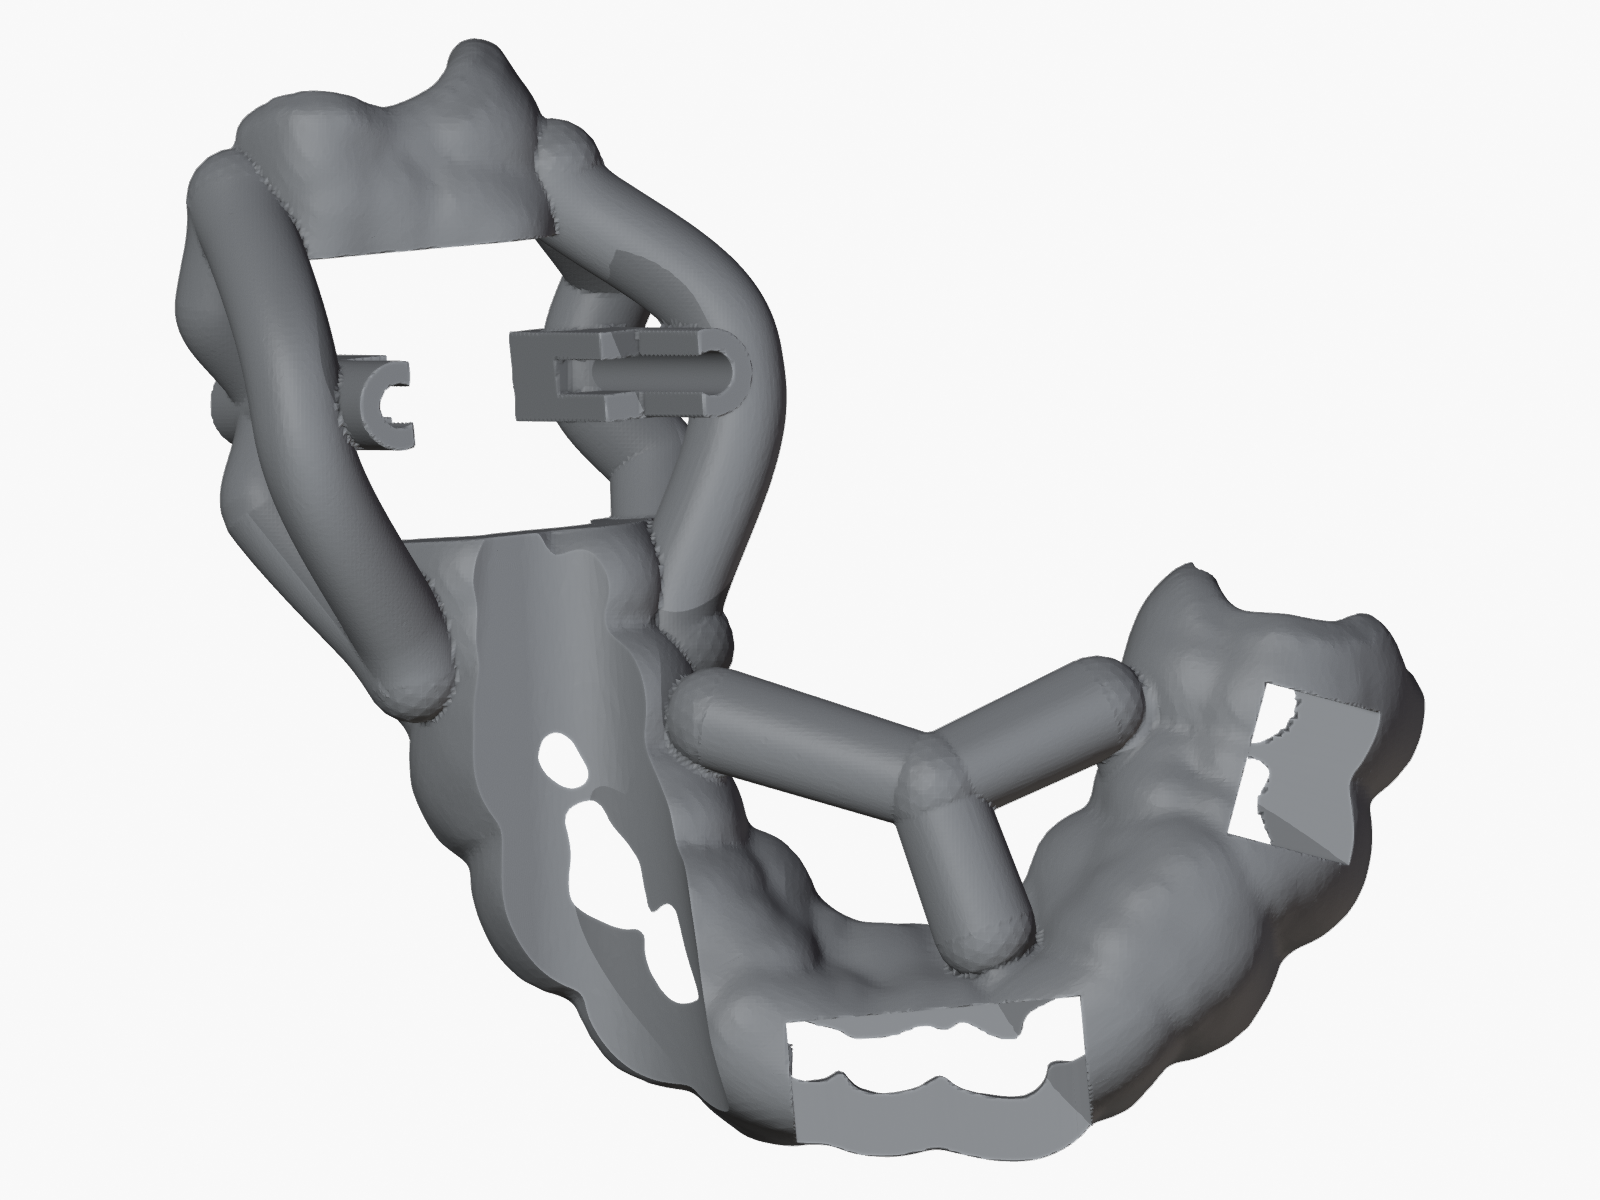
\includegraphics[width=\linewidth]{12_final_top.png}
    \caption{顶视图}
  \end{subfigure}
  \caption{tooth-47 最终结果的整体形态。可见四根环绕导管的主梁和中部三臂 Y 梁。}
  \label{fig:final-upper}
\end{figure}

\begin{figure}[H]
  \centering
  \begin{subfigure}[t]{0.48\textwidth}
    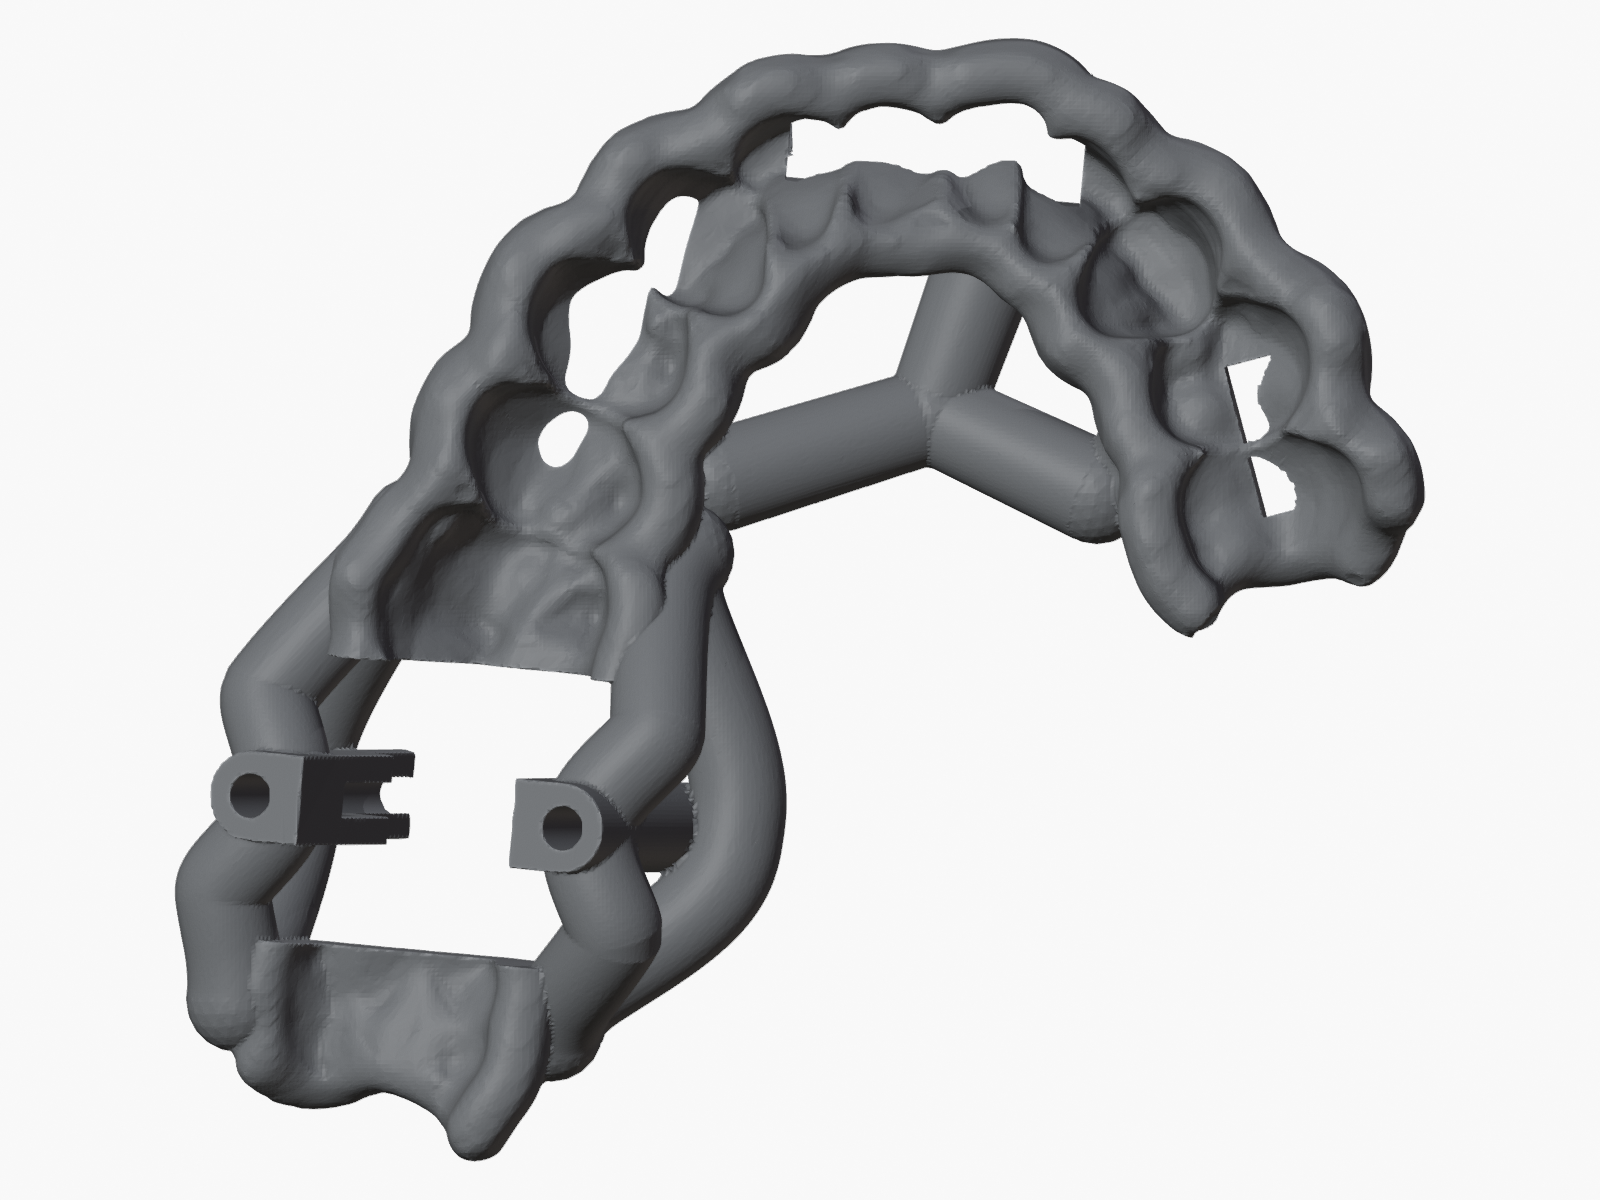
\includegraphics[width=\linewidth]{13_final_bottom.png}
    \caption{底视图：牙列贴合面与观察窗}
  \end{subfigure}\hfill
  \begin{subfigure}[t]{0.48\textwidth}
    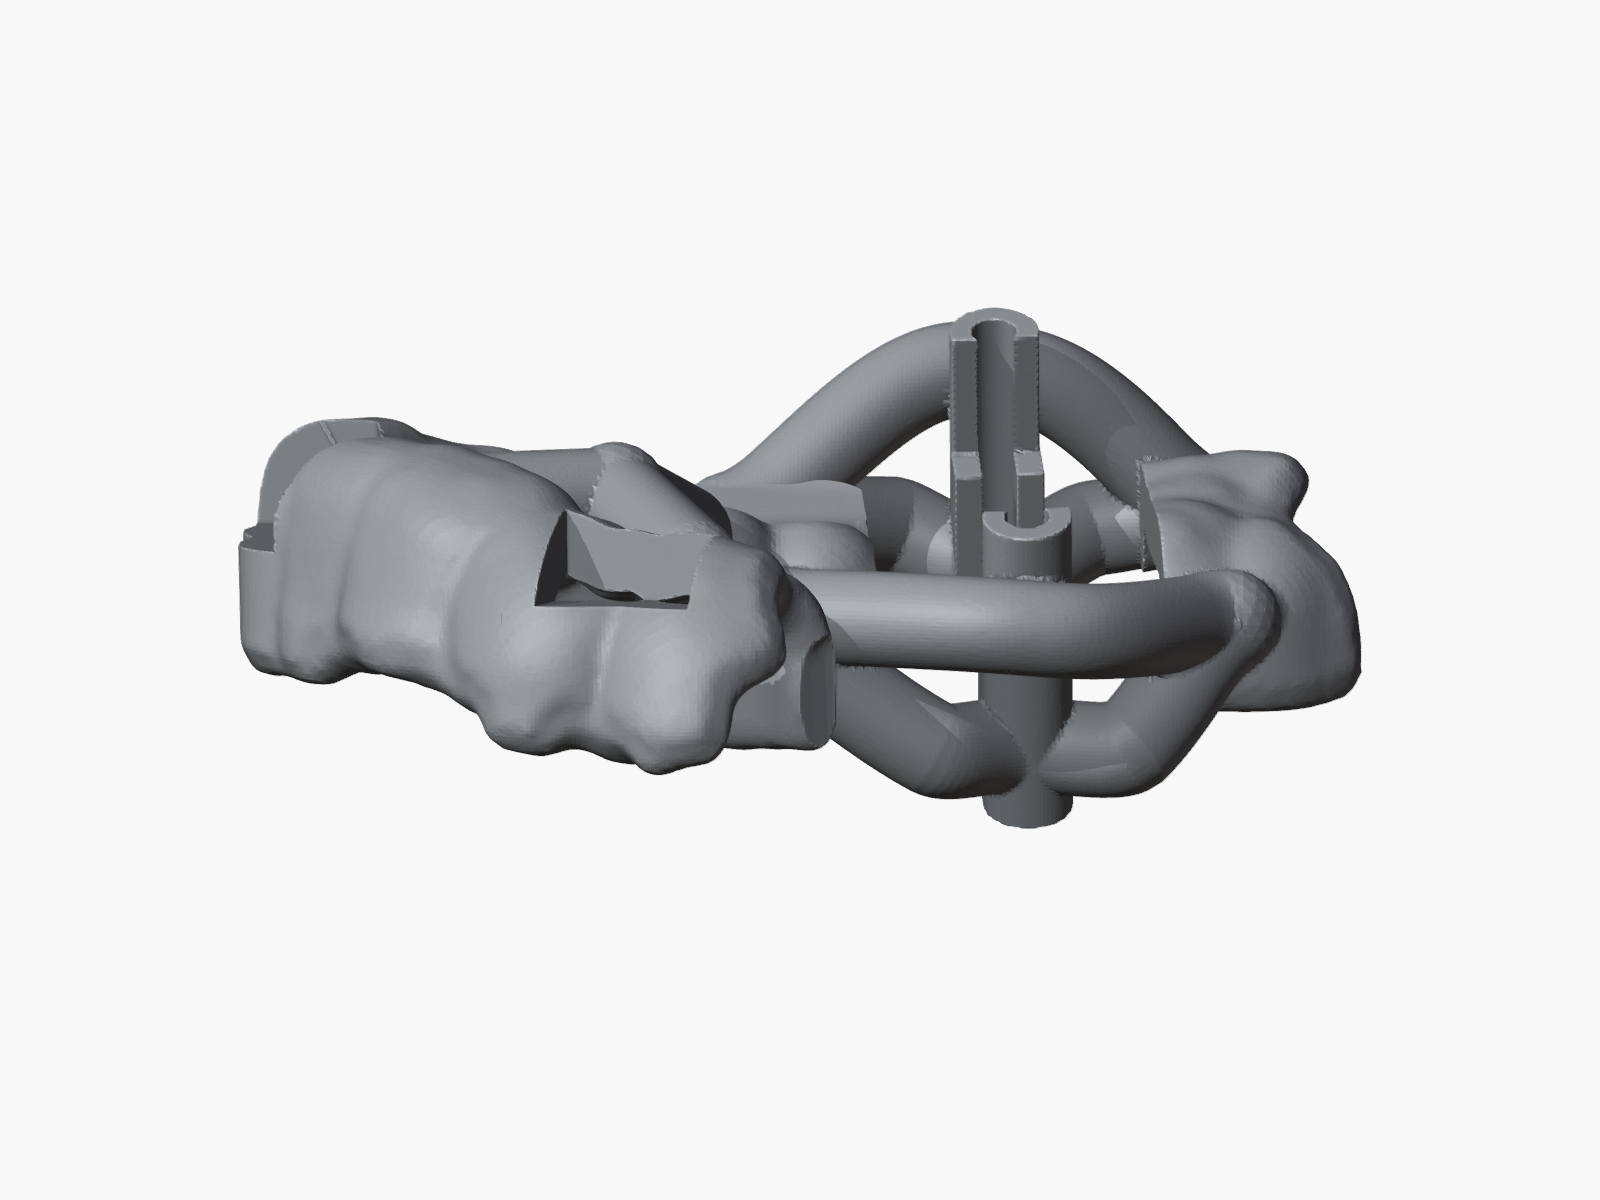
\includegraphics[width=\linewidth]{14_final_side.png}
    \caption{侧视图：导管、梁架和导板高度关系}
  \end{subfigure}
  \caption{tooth-47 最终结果的底视与侧视。}
  \label{fig:final-lower}
\end{figure}

从图中可以直观看到几个设计意图：双导管 C 口仍开放；主梁以较大弧度绕开操作区；Y 梁把
导板的三个牙位区域连成三角支撑；观察窗在贴合面形成局部开口。也能看到体素融合后的边界
不再像输入三角网格那样锐利，这是 0.2 mm 重网格带来的预期离散效果。

\section{手机避让包络}

手机旋转轴为 $(0.4439,-0.0138,0.8960)$，枢轴位于
$(-17.1631,13.7691,2.6937)$ mm。41 个姿态的角度步长为 0.25°，估算最大半步未采样位移约
0.0996 mm。最终包络为封闭体，体积约 $6660.45\,\mathrm{mm^3}$，含 1,590,056 个顶点和
3,180,108 个三角面。这个网格远比最终导板更密，是当前生成时间和内存占用的主要来源之一。

\section{最终 STL 的独立静态统计}

对现有 \projectpath{output/tooth_47/twin_guide.stl} 进行独立 Trimesh 读取，结果如下：

\begin{table}[H]
\centering
\begin{tabular}{lr}
  \toprule
  指标 & 结果\\
  \midrule
  顶点 / 三角面 & 138,861 / 277,774\\
  是否封闭 & 是\\
  绕序是否一致 & 是\\
  是否有效体积 & 是\\
  连通体数量 & 1\\
  体积 & $6670.718\,\mathrm{mm^3}$\\
  表面积 & $5981.815\,\mathrm{mm^2}$\\
  包围盒尺寸 & $59.954\times53.871\times23.953$ mm\\
  \bottomrule
\end{tabular}
\caption{现有 tooth-47 最终 STL 的静态网格统计。}
\end{table}

这些数据证明文件本身是单一闭合体，但不能替代当前配置下的完整
\texttt{generate --validate}。静态封闭并不自动证明每条梁都保留、每个孔都通畅或手机包络
已经正确切除。

\section{案例产物的版本边界}

现有最终图和 STL 的修改时间约为 2026-07-26 21:59；当前
\projectpath{blender/guide_modeling.py} 的修改时间为 2026-07-27 13:10，病例 YAML 也在
2026-07-27 00:33 更新。输出中仍名为 \projectpath{generated_sleeves.png}，而当前 YAML 已
明确为 \texttt{input} 模式；当前代码在 input 模式应输出
\projectpath{selected_input_sleeves.png}。这进一步说明现有产物与当前源码并非严格同一快照。

\begin{takeaway}
tooth-47 的中间结果足以生动解释算法，观察窗 QA 和最终 STL 静态拓扑也表现良好；正式交接
前仍应在冻结版本上重新生成一次，并把源码版本、配置摘要和验证报告与 STL 一起归档。
\end{takeaway}


\chapter{质量保证、测试体系与验收逻辑}

\section{测试层次}

项目测试约 3400 行，分为三层：

\begin{itemize}
  \item \term{单元测试}：配置解析、几何不变量、导管估计、锚点射线、Y 梁汇合点、特殊
  拓扑和文档 docstring；
  \item \term{Blender 后端测试}：封闭圆管扫掠、导管重建、体素并集、布尔差集、连通体
  清理和重复三角形检测；
  \item \term{端到端测试}：从病例配置运行生成流程，检查 STL 导出和验证结果。
\end{itemize}

单元测试特别覆盖了几个容易回归的几何决策：实心 cutter 不能被选为导管；上下 Q/P 的边缘
余量和偏移公式；U/背 U 射线角度；缺牙插值；低梁局部下潜；Y 梁 maximin 锚点；末端节点
共享；input 导管模式和 YAML 合并规则。

\section{生成阶段的失败关闭}

下列情况不会静默退化：不足两根有孔导管、导板标架退化、牙位报告 QA 不完整、上下颌或
输入路径不一致、射线找不到外壁出口、两导管内外侧差异不足、Y 梁三锚点近共线、布尔结果
不是封闭体、生产 review 状态未确认等。失败关闭能阻止几何错误进入最终 STL，但也意味着
新增病例通常需要明确修正语义和参数，不能只放宽容差。

\section{最终 STL 验证项目}

\begin{longtable}{p{0.27\textwidth}p{0.63\textwidth}}
  \toprule
  验证项 & 方法与阈值\\
  \midrule
  \endfirsthead
  \toprule
  验证项 & 方法与阈值\\
  \midrule
  \endhead
  拓扑 & 边界边、非流形边和重复三角形均为 0；恰有一个连通体。\\
  导管保留 & 参数化或输入导管表面样本位于最终体内，或距离表面不超过两个体素；保留率至少 0.90。\\
  主连接梁 & 排除孔腔内不应保留的中心线点后，中心线保留率至少 0.95；P 点和 A 点距离受限。\\
  根部强化 & 唯一导板端数量正确，球头探针和贴合脚探针具有足够包覆率。\\
  Y 梁 & 三臂中心线保留率、汇合点和应有的导板端强化。\\
  导孔 & 沿轴向自适应截面，在 0、0.5、0.9 倍可用半径上布置多角度探针；阻塞数必须为 0。\\
  观察窗 & 每条最终修正语义轴的点不在实体内，且到最近表面距离不小于 0.20 mm。\\
  特殊结构 & 根据模式检查跨分量、末端 U 梁或远中公共节点的几何公式和保留率。\\
  \bottomrule
\end{longtable}

\section{当前验证尚未覆盖的部分}

\begin{itemize}
  \item 手机包络在生成时被切除，但 \texttt{validate\_guide()} 不重新构造包络并逐点验证净空；
  \item 操作窗没有像导孔和观察窗一样形成独立、详细的最终探针报告；
  \item input 模式以配置内径作为孔道参考，不能替代对真实输入导管全孔腔的高精度计量；
  \item 结构检查主要是中心线和局部探针保留率，不直接计算有限元强度、疲劳、打印支撑或变形；
  \item 封闭和单连通不等同于没有自相交、过薄壁或不可清洁死角。
\end{itemize}

\section{本次报告构建期间的验证状态}

本次已读取现有过程报告、检查 tooth-47 图片，并用独立 Trimesh 读取最终 STL，确认其为单一
封闭有效体。尝试通过系统 Python 运行单元测试时缺少 pytest；随后尝试调用 Blender 5.2
后台测试环境，但 Blender 在启动后崩溃并写出 crash 文件，未得到可信的测试通过结果。
因此本报告不会把“测试文件存在”表述为“当前环境测试已全部通过”。

建议交接验收在稳定 Blender 环境中依次执行：文档严格构建、全部单元测试、Blender 后端
测试、tooth-47 当前版本重新生成，以及 \texttt{generate --validate}。每次运行都应保存
命令、退出码和验证 JSON。


\chapter{潜在问题、技术难点与改进建议}

\section{风险分级总览}

\begin{longtable}{p{0.09\textwidth}p{0.28\textwidth}p{0.50\textwidth}}
  \toprule
  优先级 & 问题 & 影响与建议\\
  \midrule
  \endfirsthead
  \toprule
  优先级 & 问题 & 影响与建议\\
  \midrule
  \endhead
  P0 & 版本与产物不可严格追溯 & tooth-47 输出早于当前源码/YAML，且文件名显示模式漂移。冻结版本后重跑，清单中写入 Git 提交、全部输入/配置哈希、Blender 和依赖版本。\\
  P0 & 医疗/制造验收边界不完整 & 当前 QA 是几何与拓扑检查，不等同于临床安全、打印可制造性或试戴。必须保留人工审核与实体制造验证。\\
  P1 & 手机避让未被独立复算 & 生成阶段执行差集，验证器不重建包络。增加包络净空探针、关键姿态碰撞检查和梁连续性专项报告。\\
  P1 & 观察窗失败关闭语义不完全一致 & 适配层在 QA 非全真时会记录 \texttt{retained\_after\_failed\_QA}，随后仍可能返回 cutter；与文档中“最终失败关闭”的表述存在差异。生产路径应显式拒绝失败 QA。\\
  P1 & input 模式仍经过体素融合 & “保留输入导管”是相对于不重钻孔而言，并非逐三角面原样保留。增加重采样前后 Hausdorff 距离、孔径和 C 口面积检查。\\
  P1 & 外部工作区模块未在包依赖中表达 & 牙位识别和观察窗依赖 \projectpath{tooth_guide_mapping} 与 \projectpath{scripts}，但 \texttt{pyproject.toml} 只声明 PyYAML。建议打包成显式依赖或建立版本锁定接口。\\
  P2 & 文档与病例参数漂移 & 文档写 0.2 mm/90° 与 0.5/1/2 mm 回退，tooth-47 实际为 0.5 mm 与 1/2/3 mm。由配置自动生成参数表，减少手写常数。\\
  P2 & 部分阶段仍标记 experimental & 只有导管阶段为 stable，其他阶段版本为 0.1--0.4。对每阶段建立明确稳定条件和回归病例覆盖矩阵。\\
  P2 & 操作特征识别假设较强 & 若非导管组件中没有近圆形候选，\texttt{min(circular)} 会失败；圆度阈值和“最近双导管中点”对异常装配敏感。增加清晰诊断与显式配置回退。\\
  P2 & 高密度手机包络成本很高 & tooth-47 包络超过 318 万面。考虑分层包围体、角度自适应采样、SDF/体素并集或只在导板邻域裁剪。\\
  P3 & 输出目录清理范围粗 & 每次生成会删除输出目录顶层全部 PNG/STL。保持专用运行目录，或按清单只清理本程序上次生成的文件。\\
  \bottomrule
\end{longtable}

\section{几何建模本身的难点}

\subsection{薄壳、共面和非流形网格}

牙列和导板来自扫描或上游 CAD，可能存在重复面、孔洞、自交和巨大三角形。薄壳差集尤其容易
在共面处产生碎片。项目通过体素融合提高鲁棒性，再用 manifold3d 精确复切恢复功能孔；
这是一种务实折中，但需要持续量化体素误差。

\subsection{语义方向比几何位置更难}

同一个世界坐标方向不能同时代表所有牙位的“外侧”。牙弓弯曲使局部 outward、近远中和
切向随牙位变化；如果 FDI 左右翻转，观察窗、主梁端点和特殊末端结构会一起翻转。相比
布尔失败，这类错误更危险，因为结果可能仍然是漂亮的封闭 STL。

\subsection{局部最优与整体结构}

每个锚点都可以局部可行，但四根主梁和 Y 梁组合后仍可能过近、交叉或干涉手机包络。当前
流程主要以确定性规则和少量 maximin/最短距离选择构造结果，尚未形成统一的多目标优化：
例如同时最小化梁长、曲率和体积，最大化夹角、根部面积和器械净空。

\subsection{布尔顺序是功能语义的一部分}

generated 和 input 模式的差异不是实现细节。一个错误的“最后再统一复切”会改变真实输入
导管；一个错误的“先切一次就结束”会让体素融合堵回孔道。后续重构必须用模式化测试锁定
每一步 cutter 的作用对象和顺序。

\section{建议的改进路线}

\begin{enumerate}
  \item \term{先补追溯}：每次生成写出统一 run manifest，包括源码版本、dirty 状态、输入和
  配置哈希、算法版本、命令、耗时、环境和输出哈希。
  \item \term{再补验证空白}：优先增加手机包络独立净空、操作窗终态检查，以及 input 导管
  重采样误差和真实孔径量测。
  \item \term{收紧失败语义}：任何观察窗 QA 非全真都不允许进入正式生成；警告继续的贴合脚
  应在生产模式转为明确的人工签核项。
  \item \term{建立病例覆盖矩阵}：普通、断裂导板、U 型末端、远中公共节点、相邻双种植位、
  input/generated 两模式均有固定回归与阈值。
  \item \term{控制性能}：为手机包络和观察窗记录每阶段耗时、峰值内存和网格规模，避免只在
  最终命令超时后排查。
  \item \term{自动生成文档参数}：从 dataclass 默认值和病例 YAML/JSON 生成表格，降低说明文档
  与实际配置分叉。
\end{enumerate}


\chapter{项目交接与新病例落地建议}

\section{接手项目的推荐阅读顺序}

\begin{enumerate}
  \item 先读 \projectpath{README.md} 和本报告，建立输入—规划—实体化—验证的整体认识；
  \item 阅读 \projectpath{config.py} 的数据类和 \texttt{CaseConfig.from\_json()}，理解配置
  合并、安全门和模式互斥；
  \item 以 \projectpath{generation_process.py} 为索引，逐步定位七阶段入口；
  \item 重点读 \projectpath{tooth_section_anchors.py}、\projectpath{point_linking.py} 和
  \projectpath{blender/guide_modeling.py}，它们决定锚点、中心线和最终布尔顺序；
  \item 最后读 \projectpath{guide_validation.py} 和测试，理解项目真正承诺检查什么。
\end{enumerate}

\section{新病例的建议流程}

\begin{enumerate}
  \item 将导板、牙列、双导管装配体放入规范病例目录，确认毫米单位和共同坐标系；
  \item 在 YAML 中填写上下颌、FDI 顺序、现存/缺失/排除牙、观察窗和人工确认方向；
  \item 选择 input 或 generated 导管模式，判断是否需要断裂跨接、末端 U 梁或远中公共节点；
  \item 在 YAML 中为每个主梁和 Y 梁端点指定牙位站位、侧别和射线角度；
  \item 先运行 \texttt{process}，检查牙位、T 点、射线、A 点、Q/P 和中心线；
  \item 查看牙位映射、观察窗、锚点和梁架过程图，只修正语义或明确参数，不用无限放大容差；
  \item 在专用输出目录执行完整生成，人工检查四视图和导孔/窗口；
  \item 更新 review 状态，再执行 \texttt{generate --validate}；
  \item 保存 run manifest、输入、配置、中间报告、验证结果、最终 STL 和必要图片。
\end{enumerate}

\section{问题定位顺序}

\begin{description}
  \item[锚点落到导板顶部] 检查牙合轴符号、邻牙参考切向、射线角度、外壁出口法向判定和
  导板连通分量，而不是退回轨迹百分比。
  \item[U/背 U 两点在同一侧] 检查 \texttt{local\_outward}、射线符号和 FDI 左右映射，
  不要用渲染图屏幕左右替代牙弓语义。
  \item[低梁异常弯折] 检查局部下潜两侧是否继承各自的外层曲线切向，以及 P 是否过深。
  \item[导孔堵塞] 检查当前导管模式、复切顺序、cutter 轴向范围和体素尺寸。
  \item[观察窗消失] 检查最终 profile cutter 是否复切、指纹是否失效、报告 QA 是否全真。
  \item[梁被切断] 分别检查牙列保护体和手机包络，不要只看最终网格表面。
  \item[末端方向反向] 检查 FDI 方向、参考邻牙到末端牙向量和叉积符号。
\end{description}

\section{建议的正式交付清单}

\begin{itemize}
  \item 冻结的源码版本与依赖锁文件；
  \item 病例 JSON、YAML 和所有输入 STL/JSON 的摘要；
  \item tooth mapping、观察窗和手机包络的过程报告；
  \item 锚点、切口、连接梁和最终四视图；
  \item 最终 STL 的 SHA-256、拓扑统计和完整 ValidationResult；
  \item 人工设计复核记录、制造参数和实体试戴/质检记录；
  \item 本报告及其可编译 LaTeX 源工程。
\end{itemize}

\begin{takeaway}
项目交接的重点不是记住每个默认值，而是保持三条链条完整：病例语义能追溯到锚点，锚点能
追溯到最终实体，最终实体能追溯到独立验证和人工审核。
\end{takeaway}



\appendix
\chapter{核心模块索引}

\begin{longtable}{p{0.34\textwidth}p{0.56\textwidth}}
  \toprule
  模块 & 交接时应掌握的职责\\
  \midrule
  \endfirsthead
  \toprule
  模块 & 交接时应掌握的职责\\
  \midrule
  \endhead
  \projectpath{config.py} & JSON/YAML 解析、路径解析、默认值、模式枚举、参数互斥和生产 review 安全门。\\
  \projectpath{generation_process.py} & 七阶段顺序和 \texttt{GenerationContext} 写入规则。\\
  \projectpath{case_analysis.py} & STL 导入、表面采样、导板中心/标架、导管装配体分量和操作特征。\\
  \projectpath{sleeve_generation.py} & 有孔导管候选筛选、候选对评分、C 口方向和导管模式。\\
  \projectpath{sleeve_estimation/*} & 切片、圆/轴拟合、导管参数化重建和网格质量。\\
  \projectpath{tooth_identification.py} & 外部牙位工作流调用、QA/路径/哈希检查和内存结果转换。\\
  \projectpath{observation_window_opening.py} & 轴扫掠观察窗适配、缓存指纹、局部 drop 回退和 cutter 报告。\\
  \projectpath{window_cutouts.py} & 导孔圆柱、操作窗局部标架与 observation profile 组合。\\
  \projectpath{sleeve_anchors.py} & 导管 Q/P、上下截面、壁厚限制和 input/generated 嵌入差异。\\
  \projectpath{tooth_section_anchors.py} & 牙位站位、缺牙插值、局部 U/背 U 方向、射线外壁出口和旧轨迹候选。\\
  \projectpath{template_anchors.py} & 独立锚点分端、导管配对、多种植位连续路径和特殊末端节点。\\
  \projectpath{press_beam_points.py} & 三种 Y 梁模式、汇合点、maximin 锚点和夹角检查。\\
  \projectpath{point_linking.py} & 五次 Hermite 主梁、低梁局部下潜、多接触点路径和 Y 臂。\\
  \projectpath{guide_component_bridge.py} & 两分量断裂导板的同侧双梁跨接。\\
  \projectpath{guide_terminal_u_extension.py} & 末端牙轮廓、远中方向、U 型延伸中心线和净距计划。\\
  \projectpath{terminal_distal_common_node.py} & 缺失末端牙的自由公共节点公式。\\
  \projectpath{clearance_adjustment.py} & 手机止挡几何、姿态采样、包络缓存和精确并集。\\
  \projectpath{blender/mesh_builders.py} & 圆柱、窗口、平行输运圆管、渐粗根、贴合脚和体素融合。\\
  \projectpath{blender/booleans.py} & manifold3d 差集、Minkowski 外扩、求解器回退和局部 STL 修复。\\
  \projectpath{blender/guide_modeling.py} & 过程渲染、牙列裁剪、模式化布尔顺序、导出和最终四视图。\\
  \projectpath{guide_validation.py} & 拓扑、导管、主梁、Y 梁、特殊结构、孔道和观察窗验证。\\
  \bottomrule
\end{longtable}

\chapter{能力矩阵}

\begin{table}[H]
\centering
\small
\begin{tabularx}{\textwidth}{p{0.25\textwidth}c c X}
  \toprule
  能力 & 当前接入 & 有测试入口 & 备注\\
  \midrule
  单种植位双导管 & 是 & 是 & tooth-47 为黄金病例\\
  多种植位连续路径 & 是 & 是 & 每种植位独立导管装配体\\
  input 导管 & 是 & 是 & 最后融合，但仍经体素化\\
  generated 导管 & 是 & 是 & 参数化重建并最终复切孔道\\
  FDI 牙位映射 & 是 & 间接 & 依赖工作区模块和映射 QA\\
  轴扫掠观察窗 & 是 & 过程 QA & 依赖工作区脚本\\
  三种 Y 梁 & 是 & 是 & 按模式配置\\
  断裂导板跨接 & 是 & 有结构检查 & 只处理两个主要分量\\
  末端 U 型延伸 & 是 & 是 & 依赖末端牙闭合轮廓\\
  远中公共节点 & 是 & 是 & 与 U 型延伸互斥\\
  手机左右摆动 & 是 & 生成报告 & 未进入独立验证完整复算\\
  轴向手机下压 & 否 & 否 & 当前深度固定为 0\\
  临床/打印验收 & 否 & 否 & 必须由外部流程完成\\
  \bottomrule
\end{tabularx}
\caption{当前项目能力边界。}
\end{table}


\chapter{tooth-47 参数与产物索引}

\section{导管与梁架参数}

\begin{longtable}{p{0.37\textwidth}>{\raggedleft\arraybackslash}p{0.19\textwidth}p{0.28\textwidth}}
  \toprule
  参数 & 数值 & 用途\\
  \midrule
  \endfirsthead
  \toprule
  参数 & 数值 & 用途\\
  \midrule
  \endhead
  导管内径 & 2.10 mm & 导孔规划参考\\
  导管主体外径 & 4.30 mm & 识别评分和几何参考\\
  导管总高度 & 16.373 mm & 参数化参考\\
  平台径向长度 & 2.036 mm & 参数化导管几何\\
  平台段高度 & 9.875 mm & 参数化导管几何\\
  闭合孔段高度 & 4.777 mm & 参数化导管几何\\
  内/外圆弧角 & 264.934° / 211.684° & C 型导管截面\\
  主梁/Y 梁直径 & 4.60 mm & 扫掠圆管\\
  体素融合尺寸 & 0.20 mm & 最终统一重网格\\
  梁—牙列净距 & 0.20 mm & 梁架牙列保护差集\\
  根部半径 & 2.484 mm & 标准 2.30 mm 半径的 1.08 倍\\
  根部过渡长度 & 3.00 mm & smoothstep 渐粗\\
  贴合脚主/次半径 & 3.00 / 2.20 mm & 导板根部接触面积\\
  贴合脚峰高/预埋 & 2.55 / 0.25 mm & 曲面贴合与融合\\
  \bottomrule
\end{longtable}

\section{主要输入和输出路径}

\begin{longtable}{p{0.29\textwidth}p{0.61\textwidth}}
  \toprule
  内容 & 项目内相对路径\\
  \midrule
  \endfirsthead
  \toprule
  内容 & 项目内相对路径\\
  \midrule
  \endhead
  病例 YAML & \projectpath{data/cases/single/tooth-47/case.yaml}\\
  工程 JSON & \projectpath{examples/case-tooth-47.json}\\
  原始导板 & \projectpath{data/cases/single/tooth-47/input/guide-template.stl}\\
  导管装配体 & \projectpath{data/cases/single/tooth-47/input/sleeve-assembly.stl}\\
  患者牙列 & \projectpath{data/cases/single/tooth-47/input/dentition.stl}\\
  手机与止挡 & \projectpath{data/cases/single/tooth-47/input/handpiece-01.stl}；\projectpath{handpiece-stop-01.json}\\
  牙位映射 & \projectpath{output/tooth_47/tooth_mapping/}\\
  观察窗 & \projectpath{output/tooth_47/observation_window_opening/}\\
  手机包络 & \projectpath{output/tooth_47/handpiece_avoidance/}\\
  最终 STL & \projectpath{output/tooth_47/twin_guide.stl}\\
  报告图片归档 & \projectpath{Tex/figures/}\\
  \bottomrule
\end{longtable}

\section{报告引用的内部资料}

本报告没有使用项目外文献。主要内部依据如下：

\begin{itemize}
  \item \projectpath{README.md}、\projectpath{docs/guide/technical-modeling-workflow.md}；
  \item \projectpath{docs/design/}、\projectpath{docs/process/}、\projectpath{docs/guide/}；
  \item \projectpath{src/twin_guide/} 全部 Python 源码；
  \item \projectpath{tests/} 中的单元、Blender 和端到端测试；
  \item tooth-47 的 YAML、JSON、牙位映射、观察窗和手机避让报告；
  \item tooth-47 的过程渲染、最终四视图和最终 STL 静态统计。
\end{itemize}


\end{document}
